
% blabla 
%\PassOptionsToPackage{dvipdfmx}{xcolor} %or dvipdfm 
%\PassOptionsToPackage{dvipdfmx}{graphicx} %or dvipdfm 
\RequirePackage{lmodern}
\documentclass[12pt]{book}


%\listfiles
\synctex=1% maybe security issue: draft only? 

% for buildParams to check empty: \ifdefempty
%\usepackage{etoolbox}
% for buildParams: \verbdef 
%\usepackage{newverbs}

% provdies \ifPDFTeX, \ifXeTeX and \ifLuaTeX. 
% iftutex test is true for XeTeX and LuaTeX, 
% and an ifpdf test is provided to test the PDF or DVI output mode.
\usepackage{iftex}

% provides \newboolean, \setboolean 
% is used to integrate html production with tex4ht and pdf production
% used to define texFhtLoaded and beamerLoaded 
% maybe this is not really absolute necessary 

\usepackage{ifthen}
\newboolean{texFhtLoaded}
\setboolean{texFhtLoaded}{false}

% only with pdflatex, warnings for xelatex and for lualatex 
% ifxetex, ifluatex, ifpdf
\ifpdf%
  %\usepackage{mlmodern}
\else
  \makeatletter
  \@ifpackageloaded{tex4ht}{%
    \setboolean{texFhtLoaded}{true}
  }{%
  }% tex4ht not loaded 
  \makeatother
\fi


\newboolean{beamerLoaded}
\makeatletter
\@ifclassloaded{beamer}{%
  \setboolean{beamerLoaded}{true}
}{
  \setboolean{beamerLoaded}{false}
}
\makeatother



\iftutex%
  \usepackage{fontspec}
\else
  % this seems to work with beamer also 
  \usepackage[utf8]{inputenc}
  \usepackage[T1]{fontenc}
\fi
%\usepackage{textalpha}


% absolutely necessary. 
% for document development add certain options. 
% Then remove headline and prevent this plugin from overwriting. 

\ifthenelse{\boolean{beamerLoaded}}{
  % here nothing to do. 
  % beamer loads geometry itself. 
  % The option a4paper does not make sense; 
  % one may set aspectratio in \documentclass
}{
  \usepackage[a4paper]{geometry}% option , showframe, showcrop 
}
%\usepackage{showframe} as an alternative 
\usepackage{microtype}
%\usepackage[indent,skip=0]{parskip}% used by pandoc but not good 
% special characters
\usepackage{textcomp}
\usepackage{anyfontsize}% important e.g. for beamer class 
%\usepackage{cleveref}


% used by hyperref and also to update index and glossary 
% to avoid clash because of loading with different options: 
% declare first 
% Note that without options the check is the most strict one 
\usepackage{rerunfilecheck}

% graphics 

\ifpdf%
  % for accessability with luatex
  %\usepackage{luatex85}
  % compiles for xelatex only 
  %\usepackage[tagged, highstructure]{accessibility}
  \usepackage{xcolor}  % [pdftex]  
  \usepackage{graphicx}% [pdftex] 
  % driver [hpdftex] is autodetected 
  \usepackage[destlabel]{hyperref}
  % sometimes comes in with svg import 
  \usepackage{transparent}
  % warning transparent package: 
  % loading aborted if not pdf-mode 
  % strange: according to documentation not for xelatex; 
  % seems to work anyway 
  % can be extended using l3opacity
\else
  % No PDF, includes dvi/xdv and HTML,... via package tex4ht 
  \usepackage[dvipdfmx]{xcolor}
  \usepackage[dvipdfmx]{graphicx}
  \ifthenelse{\boolean{texFhtLoaded}}{%
    \usepackage[tex4ht, destlabel]{hyperref}
  }{%
    \ifxetex%
      \usepackage[destlabel]{hyperref}
    \else
      \usepackage[dvipdfmx, destlabel]{hyperref}%[dvipdfmx]
      % lualatex: without [dvipdfmx] option did not find 
      % converter dvi to pdf or to ps
      % pdflatex: without [dvipdfmx] option dvips still works, 
      % but no converter for pdf
    \fi
  }% tex4ht not loaded 
  %\usepackage{bmpsize}% not for xelatex 
\fi%ifpdf

\ifluatex%
  \usepackage{luamplib}
  \newcommand*\inputmpcode[1]{\begin{mplibcode}input #1\end{mplibcode}}
\else
\fi

% \@ifpackageloaded{tex4ht}{%
% \usepackage[dvipdfmx]{xcolor}
% \usepackage[dvipdfmx]{graphicx}
% \usepackage[tex4ht]{hyperref}
% \usepackage{bmpsize}
% }{%
% \usepackage{xcolor}  % [pdftex]  
% \usepackage{graphicx}% [pdftex] 
% \usepackage{hyperref}% driver [hpdftex] is autodetected 
% }


%\usepackage[clear,pdf,eps]{svg}

\usepackage{import}
\usepackage{amsmath}

% synchronization between tex and pdf 
%\usepackage[active]{srcltx}
\usepackage{longtable}
\usepackage{listings}
% this is a workaround for including listings with latexmk.. 
% This can be fixed 
% - as shown below 
% - patch in package listings 
% - patch in latexmk 
% I would prefer the latter. 
\usepackage{xpatch}
\makeatletter
\newcommand*{\NewLine}{^^J}%
\xpatchcmd{\lst@MissingFileError}
{Package Listings Error: File `#1(.#2)' not found.}
{LaTeX Error: File `#1.#2' not found.\NewLine}{%
  \typeout{File ending patch for \string\lst@MissingFileError\space done.}%
}{%
  \typeout{File ending patch for \string\lst@MissingFileError\space failed.}%
}
\makeatother

\usepackage{fancyvrb}


% index and glossary
\ifthenelse{\boolean{texFhtLoaded}}{%
  \newcommand{\pkg}[1]{\texttt{#1}}% without indexing 
}{
  \usepackage{splitidx}%[split]
%  \usepackage{makeidx}
%  \usepackage{showidx}
  \makeindex
  \usepackage[toc]{glossaries}%,automake
  % , xindy or even [xindy={language=english,codepage=utf8}]
  % mainly for index and glossaries 
  %\makeglossaries% TBD: activate later
  \newcommand{\pkg}[1]{\texttt{#1}\sindex[pkg]{#1}} % TBD: this must be extracted 
  }

% high quality tables 
\usepackage{booktabs}
\aboverulesep=0ex
\belowrulesep=0ex

\usepackage{xurl}

%\makeglossary% for rerunfilecheck 

%\usepackage{etexcmds} %still later 
\ifthenelse{\boolean{beamerLoaded}}{
  % TBD: clarify this case. 
  % maybe beamer does not support indices or glossaries. 
  % 
}{
  \usepackage[nottoc, numindex, numbib]{tocbibind}
}

%\usepackage{latex-bnf}





\setacronymstyle{long-short}
% file formats 
\newacronym{pdf}{pdf}{portable document format}
\newacronym{dvi}{dvi}{device independent file format}
\newacronym{eps}{eps}{encapsulated postscript}
\newacronym{tex}{tex}{tex the format, which may also be latex}
\newacronym{html}{html}{hypertext markup language}
\newacronym{xhtml}{xhtml}{extensible hypertext markup language}
\newacronym{odt}{odt}{open document text}
\newacronym{doc}{doc}{outdated document format for MS word }
\newacronym{docx}{docx}{current document format for MS word }
\newacronym{sgml}{sgml}{Standard generalized markup language }
\newacronym{xml}{xml}{extensible markup language }
\newacronym{ptx}{ptx}{pdf/postscript tex format }% home brewed 

\newacronym{fig}{fig}{native file format for xfig }
\newacronym{gp}{gp}{Gnuplot file format}
\newacronym{png}{png}{Portable Network Graphics}
\newacronym{jpg}{jpg}{Graphics format developed by the Joint Photographic Experts Group }
\newacronym{gif}{gif}{Graphics Interchange Format, allows also animations }
\newacronym{svg}{svg}{Scalable Vector Graphics}
% latex file endings 
\newacronym{toc}{toc}{table of contents}
\newacronym{lof}{lof}{list of figures}
\newacronym{lot}{lot}{list of tables}
\newacronym{aux}{aux}{auxiliary file}
\newacronym{log}{log}{logging file (for \LaTeX{} and mpost)}
\newacronym{idx}{idx}{index file containing unsorted and multiple index entries}
\newacronym{ind}{ind}{%
index file containing sorted, unified and formatted index entries}
\newacronym{glo}{glo}{%
glossary file containing unsorted and multiple glossary entries}
\newacronym{gls}{gls}{%
glossary file containing sorted, unified and formatted glossary entries}


\newacronym{mp}{mp}{metapost}
\newacronym{ps}{ps}{PostScript}
\newacronym{mps}{mps}{metapost's postscript like output including text}
\newacronym{mpx}{mpx}{metapost tex output: texts }

% \newglossaryentry{latex}{name={latex},description={%
% A document preparation system 
% converting sources in the latex-format preferrably into pdf-output. 
% Historically, output was in \gls{dvi}-format 
% which is still used by htlatex as an intermediate format 
% to produce \gls{html} resp.~\gls{xhtml} and \gls{odt} output. 
% }}
% \newglossaryentry{htlatex}{name={htlatex},description={%
% A script which wraps latex 
% but producing (x)html and odt output instead of pdf 
% which is usual for latex. 
% }}
%\newglossaryentry{ps}{name={PostScript},description={%
%A computer language for creating vector graphics. 
%}}

% how to number the glossary in the toc? seemingly a gap in tocbibind 
\usepackage[nottoc, numindex, numbib]{tocbibind}

\title{Manual for the latex-maven-plugin and for an according ant-task }
\author{Ernst Reissner (rei3ner@arcor.de)}


\begin{document}
\maketitle

\tableofcontents
\listoffigures
\listoftables


\chapter{Introduction}

This document is created with pdflatex or that like 
with output format 
\ifpdf
pdf
\else
dvi
\fi

\LaTeX{} is a beautyful way to create printable documents, 
today in preferrably as \gls{pdf}-files, 
with a particular strength in typesetting formulae like 
%
\begin{eqnarray*}
\pi & = & \sqrt{12}\;\sum^\infty_{k=0} \frac{(-3)^{-k}}{2k+1}. 
\end{eqnarray*}
%
Here, portability of the format \gls{pdf} is a vital feature. 

This piece of software implements both an ant-task and a maven-plugin 
generating documentation of various formats from \LaTeX-files 
in an uniform way. 
Besides \gls{pdf}, these formats include the web-formats \gls{html} 
and \gls{xhtml}, 
open offices format \gls{odt}, microsoft's word formats like \gls{docx} 
and finally plain text. 

Uniformity of ant-task and a maven-plugin means in particular, 
that the settings which may be passed to the task 
and those allowed for the plugin are in a one-to-one relation. 
They are both described in Section~\ref{chap:settings}. 
\index{ant-task}
Both, the ant-task and the maven-plugin rely on the same code base 
which form the package {\tt org.m2latex.core}. 
The code specific for the ant-task is in {\tt org.m2latex.antTask} 
and that specific for the maven-plugin is in {\tt org.m2latex.mojo}. 

It is very usual to endow \LaTeX-files with figures. 
We support figures created in the \gls{fig} by the program xfig, 
figures created by the plotting utility gnuplot, 
the tex-specific graphic language metapost 
and finally figures in formats which can be included into a \LaTeX-file 
without preprocessing like \gls{png} and \gls{jpg} 
or with automatic conversion like \gls{svg}. 
Further functionality on \LaTeX{} figures can be easily added. 
If there is some need, please write an email to the author. 

The creation process supports an index, a glossry and a bibliography. 
Again, further functionality can be added by demand. 

The present manual is created by the maven-pugin or the ant-task 
described here. 
There should be no difference in the result. 
This manual is designed in a way that it covers the most important features 
but also to demand the most important features. 
That way, creating this manual is a top level test 
for the underlying software. 
The maven-plugin is somehow superior 
because it better supports the design process for the \LaTeX{} sources. 



\chapter{Installation}

Both the ant-task and the maven-plugin just direct parameters 
from ant and from maven, respectively, 
to the programs that do the proper work. 
Thus installation of the ant-task and of the maven-plugin 
requires that all needed programs are installed. 
These prerequisites are collected in Section~\ref{sec:prerequisites}. 
\index{ant-task}

\section{Prerequisites}\label{sec:prerequisites}

The ant-task is tested with 
{\tt Apache Ant(TM) version 1.9.4 compiled on September 11 2015}\index{ant}
and the maven-plugin with 
%
\index{maven}
\begin{verbatim}
Apache Maven 3.3.9 \
(bb52d8502b132ec0a5a3f4c09453c07478323dc5; 
2015-11-10T17:41:47+01:00)
\end{verbatim}
%
Both, ant and maven are written in java and require a java installation. 
The java\index{java} version used for tests 
is {\tt 1.8.0\_101, vendor: Oracle Corporation}. 


So, a java installation is the base for running either the ant-task 
or the maven-plugin. 
Also this plugin is written in java. 
To use the maven-plugin, of course maven must be installed 
and to use the ant-task, ant must be installed. 

The ant-task just passes parameters in the build file to the core 
and accordingly the maven-plugin passes parameters in the pom 
to the core of this software. 
The core just invokes various programs to do the actual work. 
\index{ant-task}

Besides plain building of documentation, 
this software also supports documentation development. 
\LaTeX{} and related programs are based on text files mainly 
and so a good editor is required for development. 
The author recommends and uses good old 
{\tt GNU Emacs 24.3.1 (x86\_64-suse-linux-gnu, GTK+ Version 3.16.7)} 
together with several packages to support 
various file formats. 
To list the available packages type 
{\tt M-x list-packages}. 
For comfortable development with \LaTeX, 
the {\tt auctex} package, version {\tt 11.88} is recommended. 
The version is displayed from within emacs 
by typing {\tt C-h v AUCTeX-version RET}. 
For an overview on {\tt auctex} see \cite{AucTeX}. 


FIXME: gnuplot-mode expects file extension gp. 
Should be made configurable. 

To edit metapost, the mode built-in mode {\tt Metamode} is used. 

Built-in mode {\tt Docview} to view pdf, ps and dvi. 

latexmk

Builtin modes bib-mode and bibtex

Built in reftex-modes

Useful: 
ac-math, auto-complete-auctex

Depending on what kinds of graphic formats are used, 
the following programs are required: 
%
\begin{itemize}
\item
To convert the \gls{fig}-files into \gls{pdf}-files, 
by default {\tt fig2dev}\index{fig2dev} is used. 
It makes sense to have {\tt xfig}\index{xfig} installed 
to create and edit fig-files, but this is not mandatory. 
\item
To convert gnuplot files into pdf-files, there is no alternative, 
to have installed {\tt gnuplot}\index{gnuplot}. 
It serves as an interpreter and also as a converter. 
Strictly speaking, only the latter functionality is required here. 
\item
To convert \gls{mp}-files into \gls{eps}-files, 
\index{mpost}\index{metapost}
the interpreter {\tt mpost} or equivalent is required. 
This comes with a standard tex-installation. 
With the standard configuration, 
the resultign eps-file can be viewed with {\tt ghostscript} 
and for developping it is recommended to have {\tt ghostscript} installed. 
\item
To include \gls{svg}-files into \LaTeX\index{svg}, 
{\tt inkscape}\index{inkscape} must be installed. 
It also serves to create and to edit svg-files. 
\end{itemize}



Currently for including pdf-files in both cases, 
the driver {\tt dvipdfmx} must be installed. 
Strictly speaking, this is required only for html-creation and related. 
Note that if no pictures created by {\tt fig2dev}, {\tt gnuplot}, 
{\tt mpost} or by {\tt inkscape} are used, of course, 
neither {\tt fig2dev} nor {\tt gnuplot}, {\tt mpost}, {\tt inkscape} 
nor {\tt dvipdfmx} is needed. 
To include graphics, the grapics bundle described in~\cite{GraX} is required, 
except for svg-files which requires the svg-package 
described in~\cite{SvgP}. 

As the set of required software depends on the graphic formats 
which shall be imported, 
it depends also on the set of ouput-formats 
to be supported: 
%
\begin{itemize}
\item
To create pdf-files from \LaTeX-files we use {\tt pdflatex} 
or some other kind of \LaTeX{} creating pdf-files 
like {\tt xelatex} or {\tt lualatex}. 
\index{pdflatex}\index{xelatex}\index{lualatex} 
\LaTeX{} uses several auxiliary programs. 
Above all {\tt bibtex} to create the bibliography 
and {\tt makeindex} for the index and {\tt makeglossaries} for the glossary. 
\index{bibtex}\index{makeindex}\index{makeglossaries}
The latter two 
also require the latex packages {\tt makeidx} and {\tt glossaries} 
described in~\cite{MkidxShIdxP} and in~\cite{GloP}. 
Note that {\tt makeglossaries} eiter invokes {\tt makeindex} 
or {\tt xindy}, depending on the parametrization of {\tt glossaries}. 
Both, {\tt makeglossaries} and {\tt xindy} are written in perl, 
which shall also be installed if a glossary is required. 

The package {\tt rerunfilecheck} is in any standard \LaTeX-installation. 
It is almost mandatory 
because this software presupposes {\tt rerunfilecheck} 
to ensure that the table of contents, list of figures, list of tables, 
the index and the glossary are up to date. 

It is standard to endow a pdf-file with hyperlinks. 
To support this, the package {\tt hyperref} is required. 

****
\item
To create \gls{html}-files, 
or to be more precise any kind of \gls{sgml} and \gls{xml}, 
from \LaTeX-files, {\tt htlatex} or alternatively {\tt htxelatex} is used. 
Currently the author is not aware of any alternative to the two. 
This includes also creating open office documents like odt-files. 
Thus open office documents are created in two steps, 
the first is to create pdf-files with the according tools, 
the second one is done by {\tt htlatex} or that like. 
\index{htlatex}\index{htxelatex}
\item
To create rtf-files, currently {\tt latex2rtf} is used. 
Note that this does not require {\tt pdflatex}. 
As a drawback, not all \LaTeX-packages are supported. 
\index{latex2rtf}
\item
MS word documents are created from open office documents via {\tt odt2doc} 
and thus require three steps 
and so the according tool chain. 
\index{odt2doc} 
\item
Finally, there is a way, to create plain text files from the pdf-files 
via {\tt pdftotext}. 
The way from \LaTeX{} to text via pdf makes sense 
because that text is well formatted math mode symbols like $\pi$. 
and because table of contents, index, glossary and that like are included. 
So, for that task, besides {\tt pdftotext} the whole toolchain to create
pdf-files is required. 
\index{pdftotext}
\end{itemize}

So to run this software, the abovementioned programs 
or at least the subset used, must be installed. 

\section{Setting pom.xml and build.xml}\label{sec:sgml}

To install the maven-plugin within a given maven project, 
the listing of a pom entry given in Section~\ref{chap:settings} 
can be added to {\tt pom.xml} and modified accordingly. 
In a default maven project, 
the default configuration is usable which creates pdf-documents and
\gls{html}-sites. 
The according entry to be added to the {\tt pom.xml} is then just 
%
\lstset{language=xml, basicstyle=\small}
\begin{lstlisting}
<!-- create html and pdf and other formats from latex -->
<plugin>
  <groupId>de.akquinet.jbosscc.latex</groupId>
  <artifactId>latex-maven-plugin</artifactId>
  <version>1.3-SNAPSHOT</version><!--uptodate?-->
  <!--artifactId>maven-latex-plugin</artifactId>
      <version>1.2</version--><!--uptodate?-->
</plugin>
\end{lstlisting}

Likewise to install the ant-task within an ant-project, 
the listing of a build file entry given in Section~\ref{chap:settings} 
has to be added to the {\tt build.xml}. 
Also working with an ant project 
conforming with maven conventions, 
no explicit configuration is needed. 
\index{ant-task}

In both cases, add configuration, 
where a deviation from the default requires to do so. 



\section{Completing the Installation}\label{sec:instComplete}

To install the maven-plugin, just type {\tt mvn clean install}. 
To install the ant-task, one has first to comment out in {\tt build.xml} 
the taskdef {\tt latex} and the target {\tt latex:cfg}. 
One may also adapt the lib-folder of the ant-installation, 
i.e.~the property {\tt antJarDir} where {\tt ant.jar} resides. 
Then just type {\tt ant clean jar} 
which creates the jar-file (property {\tt createdJar}) defining the ant-task. 
After that one may copy the created jar into folder {\tt antJarDir}, 
where ant finds it typing {\tt sudo ant install}. 
\index{ant-task}

Note that, if maven is installed, the command {\tt mvn clean install} 
also creates the jar-file {\tt createdJar} defining the ant-task. 
Also with this method, one has to copy the jar-file defining the ant-task 
later into ant's lib-folder. 

After having installed the ant-task, 
reactivate the taskdef {\tt latex} and the target {\tt latex:cfg} 
and run {\tt ant latex:cfg} to create this manual. 

Mixing ant and maven builds is not so good. 
One may always recover by just creating with maven. 

\subsubsection{Test}

\chapter{Usage of this Plugin and of this Task}\label{chap:usage}

This plugin may be used both if the \LaTeX-sources are finished 
to create the output described by them 
and also to support development of the \LaTeX{} sources. 
Accordingly, this section has two subsections. 

\section{The source files}\label{sec:sources}

The \LaTeX-files and also files included via {\tt\textbackslash input} 
are in the {\em tex-source directory}, 
\index{tex-source directory}
which is by default {\tt./src/site/tex}, 
where {\tt.} is the {\em base directory\/} of this maven-project. 
\index{base directory}
The \LaTeX-files to be compiled top level, 
typically not inputted anywhere via {\tt\textbackslash input}, 
are called {\em \LaTeX{} main files}. 
As an example, 
in the {\em tex-source directory\/} of this software, 
{\tt manualLatexMavenPlugin.tex} is a \LaTeX{} main file, 
whereas the file {\tt header.tex} is not although also a \LaTeX-file. 
% identification of the latex main file? 
\index{latex main file}

The included files may be again \LaTeX-files but also graphic files 
in various formats. 
There are four kinds of graphic formats, 
as regards the way their files are included in \LaTeX-files, 
all included in the tex-source directory. 
%
\begin{enumerate}
\item
The first can be included into \LaTeX-files directly 
via {\tt\textbackslash input}. 
These formats are essentially \LaTeX{} and are defined in an according package. 
An example is {\tt eepic} described in~\cite{EEpic}. 
\item
the second one via {\tt\textbackslash includegraphics} 
defined by the package {\tt graphicx} 
which is described in~\cite{GraX}. 
Chapter 2 therein mentions the supported drivers, 
among these also {\tt dvipdfm} and {\tt dvipdfmx}. 
It is not the package but the driver 
which decides on the support of graphic formats. 
The dvipdfm user manual,~\cite{DviPdfMx} lists the allowed formats 
metapost-output (i.e. \gls{mps}), postscript, 
\gls{pdf}, \gls{jpg} and \gls{png}. 
\item\label{it:transExp}
the third one must be transformed into a graphics format 
of one of the former two kinds using an external tool for transformation. 
Here, of course, only a limited support is possible, 
because there is a broad variety of formats. 
We have choosen the \gls{fig}-format **** citation **** because of its simplicity, 
the gnuplot format, described in~\cite{GnuPlot}, 
because it allows computation of pictures, 
likewise metapost, described in~\cite{MPost}. 
\item\label{it:transImp}
finally the fourth kind of graphics formats 
has to be transformed into one of the kinds one or two 
but unlike in type three, this is not done explicitly 
by an external tool but by a latex-package during the \LaTeX-run. 
Note that, although not required to be explicitly transformed, 
those graphics files induce additional files 
by running \LaTeX. 
Currently, there is only one single example for that, 
the \gls{svg}-format included by the package {\tt svg}. 
\end{enumerate}

The \LaTeX-files and the graphic files belonging to a \LaTeX{} main file 
are assumed to be in one single folder. 
If one file is included by two different main files, 
a link shall be used. 

Note that unlike former version, 
the current version of this software does create a working directory 
by cloning the tex-source directory. 
Instead it operates directly on the tex-source directory 
also creating intermediate files. 
Thus a file residing in the tex-source directory 
risks being overwritten by this software, 
if it does not stick to the rules. 
The rules are simple: 
For each graphic file, being transformed, 
i.e.~of types~\ref{it:transExp} or~\ref{it:transImp} above, 
additional files are created with the same name up to the suffix. 
Thus for these graphic files no file with the same name 
up to the ending is allowed. 
The same is true for the \LaTeX{} main files. 


\section{Exporting in various formats}\label{chap:stableUsage}


After having added the configuration of the plugin to the {\tt pom.xml}, 
it can be used directly invoking maven through 
{\tt mvn latex:cfg}. 
Here {\tt latex} is the (short) name of the plugin and {\tt cfg} is the target. 
It can also be interpreted as {\tt mvn $<$source$>$:$<$target$>$}: 
The source files are in {\tt latex}-format and the target-format(s) 
are read from the {\em configuration} in the pom 
({\em configuration} is what {\tt cfg} stands for). 
The goal {\tt cfg} is executed in maven's {\tt site} lifecycle by default. 

By default, the target formats are {\tt pdf} and {\tt html}. 
The following listing shows a configuration 
with the full range of output formats including in addition 
the open office document format {\tt odt}, 
the MS word-format(s) {\tt doc(x)} and {\tt rtf}
and also plain text format {\tt txt} in utf8 encoding. 
Note that the target {\tt docx} converts by default into \gls{docx} 
but may also be configured to produce the old fashioned \gls{doc} format. 
%
\lstset{language=xml, basicstyle=\small}
\begin{lstlisting}
<!-- create html and pdf and other formats from latex -->
<plugin>
  <groupId>de.akquinet.jbosscc.latex</groupId>
  <artifactId>latex-maven-plugin</artifactId>
  <version>1.3-SNAPSHOT</version><!--uptodate?-->
  <!--artifactId>maven-latex-plugin</artifactId>
      <version>1.2</version--><!--uptodate?-->
	
  <configuration>
    <settings>
      <targets>pdf, html, odt, docx, rtf, txt</targets>
    </settings>
  </configuration>
</plugin>
\end{lstlisting}

The resulting files in the given output formats 
are copied to the site directory, 
which is {\tt ./target/site} in a default maven project. 

Sometimes it is more convenient 
to specify the output formats not via the pom 
but directly on the command line. 
In particular, one may write {\tt mvn latex:pdf} to create documentation 
in pdf-format only. 
Note that the {\tt -X} switch activates debugging 
which results in a more verbose output. 
Example: {\tt mvn -X latex:cfg}. 

For creating the graphic files in the tex-source directory, 
there is a target {\em graphics}, invoked by {\tt mvn latex:grp}. 
This target does not create any output in the site directory. 
Finally,  there is another target for clearing the tex-source directory 
recursively, invoked by {\tt mvn latex:clr}. 
For more details on these two targets, see Section~\ref{sec:devel}. 

In a standard maven project, 
the above minimal configuration should be sufficient. 
Only if the folder structure deviates from the standard 
or if the \LaTeX{} sources require special configuation, 
parameters have to be given explicitly, 
because they deviate from the default values. 
Section~\ref{chap:settings} summarizes all available parameters, 
giving the default value and a description. 


For sake of uniformity, 
the name of the ant-task is {\tt latex:cfg} 
and it can be invoked via {\tt ant latex:cfg}. 
Unlike the maven-plugin, the ant-task 
does not allow to specify a target on the command line. 
The {\tt -d} switch activates debugging 
which results in a more verbose output. 
Example: {\tt ant -d latex:cfg}. 

Whereas by default the target directory and in particular 
the target site directory with all output of this plugin is deleted 
in maven's {\tt clean} lifecycle. 
As is described in more detail in Section~\ref{sec:devel}, 
this software creates target documents and also intermediate files 
in the tex source directory, at least with cleanup disabled. 
To eliminate the created files from the souce directory, 
just type {\tt mvn latex:clr}. 
By default, the goal {\tt clr} 
is also executed in maven's {\tt clear} lifecycle. 

There is an according ant-task {\tt latex:cfg} 
which can be invoked via {\tt ant -d latex:cfg}. 
FIXME: ant latex:clr has duplicate parameters. 
This can be fixed only by properties. 
Another problem is, to provide a complete subset of parameters 
which apply to {\tt latex:cfg} and to {\tt latex:cfg}, respectively. 

If this ant-task is used in an ant project 
with folder structure conforming with a maven project 
and if the \LaTeX{} sources do not require a special configuration, 
the above configuration is sufficient. 
Otherwise, parameters have to be given explicitly 
overwriting the default values. 

\section{Intermedate files, development and cleanup}\label{sec:devel}

During development, it is comfortable, 
to have the log-file in the same directory as the \LaTeX{} main file. 
Also if pdf- and tex-files are synchronized, 
also the pdf-file should be in the same directory. 
Likewise, files in graphic formats 
which cannot be included into a \LaTeX-file without conversion, 
that converted file shall be in the same directory as the original one. 
So, all files, manually created files 
and files arising from automatic conversions 
shall be in the same folder, at least during development. 
Also, typically, one wants to mix creation by this maven-plugin or ant-task 
with at least partial creation through external tools. 
For example, if writing \LaTeX-files with emacs, 
it is much more convenient, to compile the \LaTeX{} main file 
via {\tt pdflatex} from within emacs 
or to create a pdf-file from a \gls{fig}-file 
through {\tt xfig}'s export dialog, 
than using this maven-plugin or this ant-task. 
Also these tools work best, if all is in one folder. 

On the other hand, 
conventionally, in a maven project, 
sources are held in folder {\tt src}, 
whereas created files occur in the folder {\tt target}. 
Likewise for ant. 
The compromise, this maven-plugin and this ant-task take, 
is, that at the end of a run, 
at most the files present at the beginning of the run 
may be present in the source directory. 
So, this software builds in the following steps: 
%
\begin{itemize}
\item
Store a list of all files present at the beginning of a run.
\item
Process all graphics files of the formats requiring preprocessing.
\item
Determine the \LaTeX{} main files.
\item
Run the \LaTeX{} converter, e.g. the one creating pdf-output or docx-output.
\item
Copy the results into the target folder.
\item
Remove all files not present at the begin of a run, by default. 
\end{itemize}

To keep e.g. the resulting pdf, 
just create it via compilation through emacs, 
even if not all graphic files to be included are present 
or just by a {\tt touch}-command. 
Then in the next run of this plugin, 
this pdf will be re-created, 
that time complete with the graphics output. 
That way, synchronization between \LaTeX- and pdf-files is possible. 

Likewise, to keep the log-file or the aux-file, just touch it. 
This technique is really valuable for debugging. 

To keep all created files after a run of this maven-plugin, 
set the parameter {\tt cleanUp} in the pom 
to {\tt false} as illustrated in the listing below. 
For the ant-task likewise. 
%
\lstset{language=xml, basicstyle=\small}
\begin{lstlisting}
<!-- create html and pdf and other formats from latex -->
<plugin>
  <groupId>de.akquinet.jbosscc.latex</groupId>
  <artifactId>latex-maven-plugin</artifactId>
  <version>1.3-SNAPSHOT</version><!--uptodate?-->
  <!--artifactId>maven-latex-plugin</artifactId>
      <version>1.2</version--><!--uptodate?-->
	
  <configuration>
    <settings>
      <targets>pdf</targets>
      <cleanUp>false</cleanUp>
    </settings>
  </configuration>
</plugin>
\end{lstlisting}


But how can one get rid of all these newly created files? 
That is what is the target {\tt latex:clr} is for: 
It removes all created graphic files 
and for each latex main file, it removes all files with ``similar'' names. 
Typically, this suffices, to remove all files created. 
If not, please inform the developer of this software. 
Of course, if further software is used which creates additional files, 
like emacs creates a folder {\tt auto}, 
these files cannot be removed by this maven-pugin or this ant-task. 

During development of a \LaTeX-main file, 
it is often more conventient to compile from within an editor like emacs. 
The problem is, that compilation fails if the graphic files are missing. 
This is what the target {\tt latex:grp} is for: 
It creates all graphic files required to compile the \LaTeX-main files. 

Still this does not create a bibliography, an index or a glossary. 
With {\em auctex}\index{auctex}, an emacs-package for editing \LaTeX, 
bibliography and index are well supported. 
To create a glossary, auctex has to be modified a little. 

FIXME: include this into auctex. 

That way also the log-files required are created: 
In this case, the files {\tt ManualLatexMavenPlugin.xxx} 
where {\tt xxx} is {\tt log} for \LaTeX, {\tt blg} for {\tt BibTeX}, 
{\tt glg} for {\tt makeglossaries} and {\tt ilg} for {\tt makeindex}. 


rsvg-convert -f pdf -o t.pdf t.svg
inkscape t.svg --export-pdf=t.pdf
convert file.svgz file.pdf 
rasterizer -m application/pdf file.svgz -d file.pdf
cairosvg in.svg -o out.pdf
yyy

\chapter{Graphical Preprocessing}\label{chap:GraphConversions}

This section describes the conversions of 
graphical source files into target files 
in detail. 

But pdf also occurs as an intermediate format for pictures. 
For historical reasons, still \gls{eps} is used. 
Section~\ref{sec:figpdf} shows that it suffices to stick to pictures 
in pdf-format. 
% FIXME: REALLY? 
%FIXME: missing pdf als basic input format. What about (e)ps? 
Section~\ref{sec:fig2dev} shows how {\tt fig2dev} converts fig-files 
into \LaTeX-files containing text and including graphics in as pdf-files. 
Likewise, Section~\ref{sec:gnuplot2pdf} describes 
how gnuplot converts gnuplot-files into pdf-files. 
An insteresting alternative to gnuplot for computing pictures 
is metapost described in Section~\ref{sec:metapost}. 
A more elaborate alternative to fig-pictures are svg-pictures 
described in Section~\ref{sec:picSvg}
Also several formats collected in Section~\ref{sec:picasis} 
may be included as is. 



\section{Including pdf-files}\label{sec:figpdf}

Modern \LaTeX{} implementations directly create pdf-files. 
Thus it makes sense, to allow including graphics as pdf-files 
in \LaTeX-files. 
This is done in pdf mode 
by the \LaTeX-packages {\tt xcolor} and {\tt graphicx}. 
In contrast, traditionally \LaTeX{} produced output in the \gls{dvi}-format 
which is still used to create \gls{html}-output, 
this is not supported by the default driver, 
Instead it shall be used the driver {\tt dvipdfmx}. 
To obtain a \LaTeX-file which works both for creating pdf and html, 
insert in the header of the \LaTeX{} main file 
%
\lstset{language=tex, basicstyle=\small}
\lstinputlisting[firstline=9, lastline=21]{header.tex}

An alternative, which we do not use 
is replacing the pdf by an \gls{eps} via configuration file {\tt myxhtml.cfg} 
which is listed below. 
%
\lstset{language=tex, basicstyle=\scriptsize}
\lstinputlisting{myxhtml.tex}
%
It applies when converting \LaTeX{} into html and that like 
with htlatex if invoking someting like {\tt htlatex xxx.tex myxhtml,...} 
where {\tt myxhtml} is located in the same directory as the \LaTeX-file 
to be processed. 
The configuration file essentially contains a graphics configuration, 
which applies conversion to pdf-files included in the \LaTeX-file {\tt xxx.tex}
via {\tt \textbackslash includegraphics}. 


\section{Conversion of fig-files}\label{sec:fig2dev}

\index{xfig}
\index{fig2dev}
A simple but still useful tool to draw figures is {\tt xfig} 
which stores graphics in a native format 
described in \cite{XFigF} with file extionsion {\tt .fig}. 
The file extension {\tt .fig} is also used by matlab to store plots 
but this is something different. 
Graphics in xfig format cannot be directly included in latex files 
but must be exported into a \LaTeX-readable format. 

To export a file {\tt xxx.fig} into several external formats, 
{\tt xfig} uses {\tt fig2dev}. 
A look in \cite{XFigF}, Section 3.4 shows that texts with set ``special''-flag 
are interpreted as (la)tex-code. 
For these texts the appropriate export language would be {\tt latex}. 
On the other hand, {\tt latex} is weak in graphics 
and {\tt pdf} would be the ideal export format for all kinds of objects, 
except for texts with set ``special''-flag. 
In {\tt pdf} format, texts are interpreted litterally, 
independent of the ``special''-flag. 
Thus {\tt fig2dev} offers a mixed solution: 
export format {\tt pdftex} which yields a pdf-file 
containing all but text with set ``special''-flag 
and complementary {\tt pdftex\_t} which yields a tex-file 
including the pdf-file and the texts with set ``special''-flag. 
\index{special-flag}%maybe glossary 

For example, the fig-file defining Figure~\ref{fig:fig2dev}, 
{\tt 01fig2dev.fig} is transformed into a file  {\tt 01fig2dev.ptx} 
in format {\tt pdftex\_t} which starts like this: 
%
\lstset{language=tex, breaklines, basicstyle=\small}
\lstinputlisting[lastline=25]{01fig2dev.ptx}

The file {\tt xxx.ptx} is ``inputted'' to the tex-file of this manual 
by {\tt\textbackslash input\{xxx.ptx\}} 
automatically including {\tt xxx.pdf}. 
Note that the full path {\tt pppxxx.pdf} to {\tt xxx.pdf} is required, 
because relative paths are interpreted in terms of the file 
containing {\tt\textbackslash input\{xxx.ptx\}}. 
Observe also that we can drop the suffix which is expressed as ``{\tt pppxxx}'' 
because \LaTeX{} chooses the right suffix: 
for pdf-format this is {\tt.pdf}. 
As we will see below, 
leaving the suffix away is crucial to make {\tt xxx.ptx} work 
both for pdf-format and for dvi-format required to create html- and odt-files. 
As indicated in Section~\ref{sec:figpdf}, 
the commands in {\tt xxx.ptx} 
require the packages {\tt graphicx} and {\tt xcolor}. 

To export {\tt xxx.fig} into {\tt xxx.ptx} and {\tt xxx.pdf} 
requires two commands: 
%
\begin{Verbatim}[fontsize=\scriptsize]
fig2dev -L pdftex   <fig2devGenOptions> <fig2devPdfEpsOptions>           xxx.fig xxx.pdf   
fig2dev -L pdftex_t <fig2devGenOptions> <fig2devPtxOptions>    -p pppxxx xxx.fig xxx.ptx
\end{Verbatim}
%
Both commands specify the input file {\tt xxx.fig}, 
both use the options given by the parameter {\tt fig2devGenOptions} 
while each invocation allows to specify also specific options, 
{\tt fig2devPdfEpsOptions} and {\tt fig2devPtxOptions}, respectively, 
and both use the option {\tt -L} to specify the output format (``language''). 

%FIXME: ptx-->tex and then: convention: intuitive suffixes 

The parameters specific for {\tt pdftex} are called {\tt fig2devPdfEpsOptions} 
because the options available are the same 
as for output format {\tt pstex} creating eps-files. 
An example for a common option would be {\tt -b width} 
which shall specify the same boundary for both formats; 
otherwise they do not fit. 

For the output format {\tt pdftex\_t}, 
the option {\tt -p pppxxx} says, 
that the string {\tt pppxxx} must be included in {\tt xxx.ptx} 
as {\tt\textbackslash includegraphics\{pppxxx\}}. 
Note that the option {\tt-p} shall not be specified 
in {\tt fig2devPtxOptions}, because it is automatically added. 

Equivalent to mixed export with formats {\tt pdftex} and {\tt pdftex\_t} 
which is appropriate for \LaTeX-output format pdf, 
is the mixed export with the according formats 
{\tt pstex} and {\tt pstex\_t} appropriate for \LaTeX-output format dvi. 
The difference is that {\tt pstex} creates an eps-file instead of a pdf-file 
with the same content 
and {\tt pstex\_t} creates a tex-file which looks like that 
created by {\tt pdftex\_t} except including the eps-file 
instead of the pdf-file. 
If the suffix is not given, 
{\tt pstex\_t} and {\tt pdftex\_t} create identical files. 
Thus exporting {\tt xxx.fig} via 
%
\begin{Verbatim}[fontsize=\scriptsize]
fig2dev -L pstex    <fig2devGenOptions> <fig2devPdfEpsOptions>           xxx.fig xxx.eps   
fig2dev -L pdftex   <fig2devGenOptions> <fig2devPdfEpsOptions>           xxx.fig xxx.pdf   
fig2dev -L pdftex_t <fig2devGenOptions> <fig2devPtxOptions>    -p pppxxx xxx.fig xxx.ptx
\end{Verbatim}
%
and ``inputting'' {\tt xxx.ptx} works for both \LaTeX{} output formats. 


Note that {\tt xfig} chooses its file endings 
according to Table~\ref {tab:xfigSuffixes} 
which deviate from those used here. 

\begin{longtable}{|l|lll|}
\hline
Output format (language) & xfig suffix & our suffix & format \\
pstex                    & pstex       & eps        & eps \\
pstex\_t                 & pstex\_t    & ptx        & tex \\
pdftex                   & pdf         & pdf        & pdf \\
pdftex\_t                & pdf\_t      & pdf        & pdf \\
\hline
\caption{\label{tab:xfigSuffixes} Suffixes used by xfig as opposed to suffixes
  used here and actual file format }
\end{longtable}


Maybe xfig is intended to export from within the export dialog 
and not directly via a script like {\tt fig2dev}. 
This may be the reason 
why the magnification must be set in the export dialog, 
but it is stored in the fig-file nevertheless. 

Figure~\ref{fig:fig2dev} shows the transformation 
of figures with {\tt fig2dev} 
and the inclusion of the eps-file and of the pdf-file in the ptx-file. 
Note that the {\tt fig2dev}-command is configurable 
via the parameter {\tt fig2devCommand}, 
but there will be hardly any command with the same command line interface 
performing exactly the transformations given in Figure~\ref{fig:fig2dev}, 
except {\tt fig2dev} itself. 

At the same time, Figure~\ref{fig:fig2dev} is an example 
for a \LaTeX-file {\tt xxx.ptx} created from a fig-file 
and embedded in this \LaTeX-file 
with the {\tt\textbackslash input}-command. 
More than that, 
Figure~\ref{fig:fig2dev} describes the way it has been created. 
Note that all text labels are specified with set ``special''-flag, 
and are thus included as \LaTeX-text, 
except the text {\bf\tiny postscript} 
which is typeset with a postscipt font to make the difference visible. 


\begin{figure}[htb]
\begin{center}
\input{01fig2dev.ptx}
\end{center}
\caption{\label{fig:fig2dev}Conversion of a fig-file 
into pdf-, eps- and ptx-files with inclusions}
\end{figure}


\section{Conversion of gnuplot-files}\label{sec:gnuplot2pdf}

This software supports plots drawn with {\tt gnuplot}, or, to be more precise, 
figures stored in .gp-files created by {\tt gnuplot}. 
Note that there seems to official file extension 
to identify gnuplot files. 
From the most common extensions {\tt.plt}, {\tt.gpi} and {\tt.gp} 
we have choosen the one with the least collision 
and supported by emacs and by my file browser: {\tt.gp}. 
% FIXME: should be configurable. 
To export a file {\tt xxx.gp} into several external formats, 
it uses {\tt gnuplot} itself. 
% FIXME: look at https://www.file-extensions.org/
According to the manual~\cite{GnuPlot}, Part IV, 
{\tt gnuplot} supports output formats through so called {\em terminals}. 
Among those are several ones intended for inclusion into latex-files, 
like {\tt Cairolatex}, {\tt Eepic}, {\tt Epslatex}, {\tt Latex}, {\tt Lua}, 
{\tt Mf}, {\tt Mp}, {\tt Postscript}, {\tt Ps(la)tex}, {\tt Pstricks}, 
{\tt Texdraw} and {\tt Tpic}. 
Note that also export into the fig-format via the terminal {\tt Fig} 
is supported which in turn may be included in latex 
as described in Section~\ref{sec:fig2dev}. 
Also {\tt gnuplot} pictures may be exported in metapost format 
which in turn may be included in latex 
as described in Section~\ref{sec:metapost}. 

This software supports only the export via the terminal {\tt Cairolatex} 
which offers export to mixed pdf and \LaTeX: 
graphics in pdf and text in \LaTeX{}
which yields the fonts typical for \LaTeX{} 
as described for fig-files in Section~\ref{sec:fig2dev}. 

Accordingly, the export yields two files 
but unlike for fig-files these are created with a single command: 
%
\begin{verbatim}
gnuplot -e "set terminal cairolatex pdf <gnuplotOptions>;
            set output 'pppxxx';
            load 'xxx.gp'"
\end{verbatim}
%
exports {\tt xxx.gp} to {\tt xxx.ptx} and to {\tt xxx.pdf}, 
the former containing \LaTeX{} and including the latter 
using options given by the parameter {\tt gnuplotOptions}. 
As described for exporting fig-files in Section~\ref{sec:fig2dev}, 
the output must be specified with the full path and without ending. 

Accordingly, 
%
\begin{verbatim}
gnuplot -e "set terminal cairolatex eps <gnuplotOptions>;
            set output 'pppxxx';
            load 'xxx.gp'"
\end{verbatim}
%
exports {\tt xxx.gp} to {\tt xxx.ptx} and to {\tt xxx.eps}, 
the former containing \LaTeX{} and including the latter 
using options given by the parameter {\tt gnuplotOptions}. 
Note that this writes another but identical file {\tt xxx.ptx}. 
Thus performance is not optimal, but {\tt gnuplot} offers no way to avoid this. 
If being strict, {\tt xxx.ptx} is perfectly correct only for output {\tt eps}, 
if comments and error messages are taken into account 
but as long as no error occurs, the result is perfectly ok also for {\tt pdf}. 

As for inclusion of fig-files, 
packages {\tt graphicx} and {\tt color} are needed. 


%FIXME: 
%Here further options are missing: 
%   // set terminal pdf {monochrome|color|colour}
%    //                      {{no}enhanced}
%    //                      {fname "<font>"} {fsize <fontsize>}
%    //                      {font "<fontname>{,<fontsize>}"}
%    //                      {linewidth <lw>} {rounded|butt}
%    //                      {solid|dashed} {dl <dashlength>}}
%    //                      {size <XX>{unit},<YY>{unit}}

Figure~\ref{fig:gp2pdf} shows the transformation of the plots 
and the inclusion of graphic files. 
In addition, Figure~\ref{fig:gnuplot} shows an example of a \LaTeX-file 
created from a gnuplot file 
and embedded in this \LaTeX-file with the {\tt\textbackslash input}-command. 
%Note that the {\tt gnuplot}-command is configurable 
%via the parameter {\tt gnuplotCommand}, 
%but there will be hardly any command with the same command line interface 
%performing exactly the transformations given in Figure~\ref{fig:gp2pdf}, 
%except {\tt gnuplot} itself. 

\begin{figure}[htb]
\begin{center}
\input{02gp2pdf.ptx}
\end{center}
\caption{\label{fig:gp2pdf}Conversion of a gnuplot-file 
into pdf-, eps- and ptx-files with inclusions}
\end{figure}

\begin{figure}[htb]
\begin{center}
\input{03someGnuplot.ptx}
\end{center}
\caption{\label{fig:gnuplot}
Converted sample gnuplot-file into ptx and pdf files }
\end{figure}


\section{Inclusion of Metapost files}\label{sec:metapost}

A graphic format, very native to TeX is {\tt metapost}, 
a derivative of {\tt metafont} originally used to describe shape of fonts. 
Although seemingly supported by \TeX{} only, 
{\tt metapost} is interesting at its own, 
as it is a graphical programming language, 
Turing complete, much like postscript. 
Files containing {\tt metapost} have the ending {\tt .mp}. 
Note that there are other graphic formats 
like monochrome pictures in TIFF-format 
which are identified with the same extension 
but the metapost format has nothing to do with this. 

The interpreter for {\tt metapost} 
is given by the parameter {\tt metapostCommand} 
which defaults to {\tt mpost}. 


Figure~\ref{fig:mp2mps} illustrates how {\tt mpost} converts an \gls{mp}-file 
{\tt xxx.mp} by default: 
%
\begin{itemize}
\item
into one or more \gls{mps}-files {\tt xxx1.mps}\dots {\tt xxxn.mps}, 
(as the mp-file may declare more than one figure) 
\item
creating a log-file {\tt xxx.log} much like \LaTeX{} does 
\item
and an \gls{mpx}-file {\tt xxx.mpx} containing the text of the figure. 
\end{itemize}

The mps-files look like postscript, or more like encapsulated postscript, 
but are not completely valid, since the prologue is missing, by default. 
Inserting the line {\tt prologues := 2;} in the first line of the mp-file 
solves the problem as~\cite{MPost}, Section 14.2.1 explains. 
Then it can be viewed in ghostscript. 

A much better alternative is to specify the the option 


Roughly speaking, the mpx-file contains text parts of the mp-file; 
more knowledge is not necessary, as the texts are also in the mps-files 
and so the mpx-file is not used by this software. 

\begin{figure}[htb]
\begin{center}
\input{04mp2mps.ptx}
\end{center}
\caption{\label{fig:mp2mps}Conversion of a metapost-file into an mps-file}
\end{figure}


Figure~\ref{fig:metapost} gives an example of a metapost file 
included in this \LaTeX-file as ab mps-file 
created from the metapost file 
and embedded in this \LaTeX-file 
with the {\tt\textbackslash includegraphics}-command. 

\begin{figure}[htb]
\begin{center}
\includegraphics{05someMetapost1.mps}
\end{center}
\caption{\label{fig:metapost}
Converted sample metapost-file included as mps-file  }
\end{figure}

Note that {\tt metapostCommand} may also besides \gls{eps} 
output \gls{svg} and \gls{png}, 
just by setting 
%
\begin{verbatim}
outputformat:="svg" 
\end{verbatim}
%
or that like 
(caution: case sensitive, assuming silently {\tt eps} if not recognized). 
One would also adapt 
%
\begin{verbatim}
outputtemplate:="\%j\%c.svg"
\end{verbatim}
%
to control the names of the mps-files created. 
Here {\tt\%j} represents the jobname and $\%c$ the number. 
One may well define alternatively 
%
\begin{verbatim}
outputtemplate:="\%j-\%c.svg"
\end{verbatim}

Finally we may set: 
%
\begin{verbatim}
prologues := 3;
\end{verbatim}

So the mp-file starts 
%
\lstset{language=metapost, basicstyle=\normalsize}
\begin{lstlisting}
outputformat:="svg";
outputtemplate:="\%j\%c.svg";
prologues := 3;
\end{lstlisting}

As an alternative, {\tt mpost} compiler may be invoked with option 
%
\begin{verbatim}
-s<key>=<value>
\end{verbatim}
%
described in~\cite{MPost}, Appendix B.2.1. 
That way we can set internal variables with values 
overwriting those given by the mp-files. 
We recommend specification of internal variables through options 
if required globally. 

This would lead to invocation 
%
\begin{Verbatim}[fontsize=\scriptsize]
mpost -s 'outputformat="svg"' -s 'outputtemplate:="%j%c.svg"' -s prologues=3 file.mp
\end{Verbatim}

%FIXME: 
Note that the output 

\section{Inclusion of svg-files}\label{sec:picSvg}

Comparable with the xfig-format described in Section~\ref{sec:fig2dev} 
but much more elaborate and widely used is the \gls{svg}-format. 
There is a huge up-to-date official SVG 1.1 specification, \cite{Svg11} 
and a specification for SVG Tiny 1.2, 
\cite{Svg12Tiny} which is itself quite short and more readable 
and gives also a good overview for ``SVG Big''. 
For a tutorial, see \cite{SvgTut}. 
As stated in \cite{Svg12Tiny}, Section 1.1, 
svg-files may contain vector graphics, raster images and text. 
It may also contain video and audio elements 
and may be interactive and dynamic, 
which goes beyond what can be included in \LaTeX. 

Figure~\ref{fig:svgWithText} shows a picture in \gls{svg}-format. 
As pdf-files can be included directly 
via the {\tt\textbackslash includegraphics}-command, 
using the \LaTeX-packages {\tt xcolor} and {\tt graphicx} 
virtually, 
{\tt xxx.svg} can be included directly via 
% FIXME: done differently 
\begin{verbatim}
%\includesvg[width=0.5\textwidth]{xxx}%
\end{verbatim}
%
using the \LaTeX-packages {\tt svg} described in~\cite{SvgP}. 
Note that the suffix of the filename shall be omitted. 

A closer look shows, that graphic preprocessing is done behind the scenes 
in the course of a \LaTeX-run 
creating files {\tt xxx.pdf} and {\tt xxx.pdf\_tex}. 
As described for fig-files in Section~\ref{sec:fig2dev} 
and for gnuplot-files in Section~\ref{sec:gnuplot2pdf}: 
The latter is a latex-file containing text 
and including the former. 
To include {\tt xxx.pdf} 
of course the \LaTeX-packages {\tt xcolor} and {\tt graphicx} 
are required. 
Moreover, it may happen that the \LaTeX-package {\tt transparent} 
is required also, depending on the features used in{\tt xxx.svg}. 

As indicated in \cite{SvgP}, Section 1, 
the {\tt svg}-package delegates the transformation 
of {\tt xxx.svg} {\tt xxx.pdf} and {\tt xxx.pdf\_tex} 
to {\tt inkscape}. 
This is a graphical editor with export functions 
which can be invoked in batchmode also. 
Of course using the {\tt svg}-package has the advantage 
that no explicit preprocessing is required, 
the created files updated by need. 
It is worth thinking about whether it is worthwile 
writing according packages {\tt fig} and {\tt gnuplot}. 

On the other hand, 
this breaks the workflow this software normally applies to graphic files. 
In particular, the package creates latex main files 
which are not removed after the latex run 
if parametrized accordingly or if something goes wrong. 
Also, the {\tt svg}-package does not provide the full flexibility 
of a standard solution. 
Since this software is still under construction 
and more than that, is in an experimental phase, 
we provide explicit preprocessing of svg-files using {\tt inkscape}. 
Another problem with the {\tt svg}-package is, 
that according to cite{SvgP}, Section 1, 
it does not work on windows platforms. 


According to \cite{SvgIncl}, Section~2.4.1, 
incscape exports mixed pdf and latex if invoked approximately as 
%
\begin{Verbatim}[fontsize=\normalsize]
inkscape -D -z --export-pdf=xxx.pdf --export-latex xxx.svg 
\end{Verbatim} 
%
Also \cite{SvgIncl}, Section~3 indicates how to input the created file 
{\tt xxx.pdf\_tex} into the latex document: 
%
\begin{verbatim}
\def\svgwidth{0.5\textwidth}
\input{xxx.pdf\_tex}%
\end{verbatim}

To obtain a unified conversion as defined in Sections~\ref{sec:fig2dev} 
and \ref{sec:gnuplot2pdf}, 
inkscape is invoked in a way to have the included pdf/eps-files 
without suffix as follows: 
%
\begin{Verbatim}[fontsize=\normalsize]
inkscape -D -z --export-pdf=xxx --export-latex xxx.svg 
inkscape -D -z --export-eps=xxx --export-latex xxx.svg 
\end{Verbatim} 

Since both the pdf-file and the eps-file are given without suffix, 
the resulting tex file is not {\tt xxx.pdf\_tex} and {\tt xxx.eps\_tex} 
but in both cases just {\tt xxx\_tex} 
as illustrated in Figure~\ref{fig:svg2pdf}. 
To obtain the correct suffixes, 
after conversion the target files must be moved accordingly. 

\begin{figure}[htb]
\begin{center}
\input{06svg2pdf.ptx}%
\end{center}
\caption{\label{fig:svg2pdf}Conversion of an svg-file 
into pdf-, eps- and ptx-files with inclusions}
\end{figure}


\begin{figure}[htb]
\begin{center}
\def\svgwidth{0.5\textwidth}
\input{07someSvg.ptx}%
%\includesvg[eps,width=0.5\textwidth]{06someSvg}%
\end{center}
\caption{\label{fig:svgWithText}Some svg-picture with text FIXME: uniformity  }
\end{figure}



\section{Pictures which are not created}\label{sec:picasis}

Figure~\ref{fig:asIsJpg} shows some picture included as jpg. 
This is done as usual with {\tt\textbackslash includegraphics}. 
Note that both for {\tt pdflatex} and siblings creating pdf-output 
and for {\tt htlatex} in conjunction with {\tt dvipdfmx} 
(see Section~\ref{sec:figpdf}) 
files in the format pdf, \gls{png}, \gls{jpg} are supported. 
 **** what about \gls{gif}? 
This list may be incomplete. 

\begin{figure}[htb]
\begin{center}
%\setkeys{Gin}{width=0.9\textwidth}
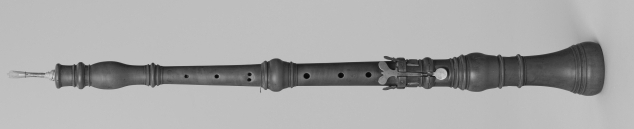
\includegraphics[width=0.9\textwidth]{08someJpgOboeBaroqueDennerMIR370}%.jpg
\end{center}
\caption{\label{fig:asIsJpg}Some jpg-picture, directly included }
\end{figure}

As an example, Figure~\ref{fig:asIsPng} shows the same picture 
as png-file. 

fixme: at the moment, htlatex does not work with pictures at all. 

\begin{figure}[htb]
\begin{center}
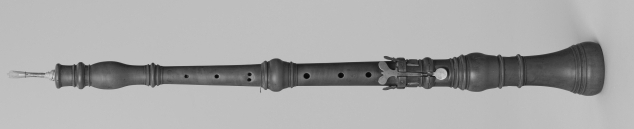
\includegraphics[width=0.9\textwidth]{09somePngOboeBaroqueDennerMIR370}%.png
\end{center}
\caption{\label{fig:asIsPng}Some png-picture, directly included }
\end{figure}



\chapter{Processing of \LaTeX{} main files}\label{chap:latexMainConversions}

Given graphics in formats includable in tex-files, 
which may require preprocessing described in 
Section~\ref{chap:GraphConversions}, 
this section describes the conversions of latex main files 
into target files in detail. 
The most important target file formats is \gls{pdf}. 
Conversion in this format is described in Section~\ref{sec:tex2pdf}. 
Note that \gls{pdf} also occurs as source format 
for included pictures and as intermediate files. 
Specific for \LaTeX{} is the \gls{dvi} format, 
which is supported mainly for historical reasons. 
% FIXME: nowhere described. 

Almost independent of the format created, 
Inclusion of bibliographies, indices and glossaries 
requires additional conversions 
done by several auxiliary programs. 
Bibliographies are described in Section~\ref{sec:bibtex}, 
indices in Section~\ref{sec:indices} 
and glossaires in Section~\ref{sec:glossaries}. 
Sections~\ref{sec:rerunMakeIndexGlossaries} 
and~\ref{sec:rerunLatex} 
are special in that they describe rerunning several programs, 
which may be necessary even if certain lists are present 
like table of contents list of figures or list of tables. 


Besides the output formats traditional for \LaTeX, 
\gls{pdf} and \gls{dvi} describing e.g. books, 
Section~\ref{sec:tex2html} describes creation of 
\gls{html}, Section~\ref{sec:tex2odt} the creation of \gls{odt} and 
Section~\ref{sec:tex2doc} creation of MS word formats like \gls{docx}. 
Finally, also pure text can be generated 
as described in Section~\ref{sec:tex2txt}. 




\section{Transforming (la)tex-files into pdf-files}\label{sec:tex2pdf}

The next step is to create a pdf-file from the tex-files. 
\LaTeX{} distinguishes master tex-files from tex-files intended to be inputted
from elsewhere. 
Master tex-files have the form 
%
\lstset{language=tex, basicstyle=\small}
\begin{lstlisting}
\documentclass{...}

\begin{document}
...
\end{document}
\end{lstlisting}

To satisfy this task, one may apply a \LaTeX{} to pdf converter {\tt latex2pdf} 
to a master tex-file {\tt xxx.tex}. 
The \LaTeX-to-pdf converter {\tt latex2pdf} 
is configurable via the parameter {\tt latex2pdfCommand}. 
Possible values are {\tt pdflatex}, {\tt lualatex} and {\tt xelatex}, 
where the first is the default for which this software is also tested. 
It is also possible to pass parameters to the \LaTeX{} to pdf converter. 

In fact, the converter {\tt latex2pdf} 
does much more than converting tex to pdf. 
Figure~\ref{fig:tex2pdf} shows for {\tt latex2pdf} set to {\tt pdflatex}, 
that besides the pdf-file also a log-file and an aux-file is created. 
The log-file contains logging information on the run of the conversion 
and the aux-file transports information from one run to the next. 
Thus conversion goes without it but it is read if present. 
This is why it is depicted at input side in dashed lines. 

What is in fact in the aux-file depends on the package. 
Among other information, 
also citations and the location of the bibliography file with ending bib 
are present. 
This cannot be used directly in the next {\tt latex2pdf} run 
to create the bibiography, 
because the entries must be retrieved from the bib-file, 
collected and sorted. 
This is done by invoking {\tt bibtex} between two {\tt latex2pdf} runs. 
Based on the aux-file, {\tt bibtex} creates a bbl-file 
containing the bibliography, which is read in in the next {\tt latex2pdf} run. 
For details see Section~\ref{sec:bibtex}. 

If an index is demanded, in addition {\tt latex2pdf} creates an \gls{idx}-file. 
As the citations, it cannot be used directly to create an index in
the next {\tt latex2pdf} run, 
because the index entries must be collected and sorted before. 
This is done by invoking {\tt makeindex} between the two {\tt latex2pdf} runs. 
Based on the idx-file, {\tt makeindex} creates an \gls{ind}-file 
containing the index, which is read in in the next {\tt latex2pdf} run. 
For details see Section~\ref{sec:indices}. 

If a glossary is demanded, this can be read off the \gls{aux}-file 
and a \gls{glo}-file is created. 
As the index, it cannot be used directly to create a glossary in
the next {\tt latex2pdf} run, 
because the glossary entries must be collected and sorted before. 
This is done by invoking {\tt makeglossaries} 
between the two {\tt latex2pdf} runs. 
Based on the glo-file, {\tt makeglossaries} creates a \gls{gls}-file 
containing the glossary, which is read in in the next {\tt latex2pdf} run. 
For details see Section~\ref{sec:glossaries}. 

In addition, 
if a table of contents, a list of figures or a list of tables is required, 
also a toc-file, a lof-file and a lot-file is created 
collecting the according information. 
If such a file is present, it is read in 
and is used to create a table of contents, a list of figures and of tables 
in the second run of {\tt latex2pdf}. 

To summarize, 
if a table of contents, a list of figures, a list of tables or 
a bibliography, an index or a glossary is present, 
a second \LaTeX{} run is required to make them appear in the pdf-output. 

If a table of contents and at the same time 
a bibliography, an index or a glossary is present, 
even two further \LaTeX{} runs are required: 
After the first one, the bibliography, the index or the glossary 
occurs in the pdf-file but not yet in the table of contents. 
This happens after the second additional \LaTeX{} run. 
As described in Sections~\ref{sec:rerunMakeIndexGlossaries} and 
\ref{sec:rerunLatex}, 
further runs of {\tt makeindex}, {\tt makeglossaries} 
and of the \LaTeX-processor {\tt latex2pdf} may be necessary. 

\begin{figure}[htb]
\begin{center}
\input{10tex2pdf.ptx}
\end{center}
\caption{\label{fig:tex2pdf}Conversion of a tex-file into a pdf-file 
(accordingly into a dvi-file)}
\end{figure}

\section{Bibliographies}\label{sec:bibtex}

In case the \LaTeX{} to pdf converter writes bibliographic information, 
into its aux-file, a bibliography must be generated. 
Bibliographic information are 
citations, a link to the bib-file containing the bibliography data, 
and optionally a link to the bibliography style file. 

To create a bibliography, a {\tt bibtex}-command must be run after the \LaTeX{} run. 
Essentially, {\tt bibtex} extracts the citations in the aux-file, 
unifies them, 
retrieves the according entries from the bib-file, sorts these 
and writes them into a bbl-file 
which can be included in the next run of {\tt latex2pdf}. 
Note that after a {\tt bibtex}-run, 
two \LaTeX{} runs are required: 
The first one just puts the bibliography in the bbl-file into the pdf-file 
and the labels of the citations into the aux-file. 
The second run places the labels at the citations 
(and puts the bibiliography
into the table of contents if there is one). 

This software presupposes, that {\tt bibtex} reads the aux-file 
and creates a bbl-file and also an blg-file with logging output 
as illustrated by Figure~\ref{fig:aux2bbl}. 
From the blg-file this software may determine 
whether {\tt bibtex} emitted an error or warnings. 


\begin{figure}[htb]
\begin{center}
\input{11aux2bbl.ptx}
\end{center}
\caption{\label{fig:aux2bbl}
Conversion of an aux-file into a bbl-file using a bibliography}
\end{figure}

Vital information on {\tt bibtex} can be found in~\cite{BibPat} 
and in~\cite{BibMar}. 
Also Chapter 10 in~\cite{Gra} gives vital information on {\tt bibtex}. 


\section{Indices}\label{sec:indices}

Note that despite of the headline of this section, 
this software supports a single index only and this requires 
the package {\tt makeidx} described in~\cite{MkidxShIdxP}. 
For an extension see Section~\ref{chap:gaps}. 

Interesting enough, 
the commands {\tt\textbackslash index} and {\tt\textbackslash makeindex} 
work even without using the package {\tt makeidx}. 
The former essentially does nothing without the latter
but if the latter is present, if {\tt xxx.tex} is the \LaTeX{} main file, 
the former writes an according entry in a file {\tt xxx.idx}. 
Essentially, 
{\tt\textbackslash makeindex} prepares writing to the \gls{idx}-file, 
whereas {\tt\textbackslash index} performs writing a line. 
For example {\tt\textbackslash index\{ant-task\}} creates an entry 
%
\begin{verbatim}
\textbackslash indexentry\{ant-task|hyperpage\}\{3\}
\end{verbatim}
%
in {\tt xxx.idx}. 
Note that {\tt xxx.idx} typically contains entries more than once 
and that the entries are not sorted. 
 
Running, the {\tt makeindex}-command performs sorting, formatting 
and typically also unification. 
Essentially, {\tt makeindex} sorts and combines index entries. 
This software presupposes, that {\tt makeindex} converts the idx-file 
into an ind-file containing the index 
and creating also an ilg-file with logging output 
as shown in Figure~\ref{fig:idx2ind}. 
From the ilg-file this software may determine 
whether {\tt makeindex} emitted an error or warnings. 

The package {\tt makeidx} provides a single command, 
{\tt\textbackslash printindex} which reads in the ind-file 
and prints the index in a separate section, 
typically at the end of the pdf-file. 
The package {\tt tocbibind} described in~\cite{TocBibIndP}, 
then writes the headline of the index into the table of contents. 
\index{table of contents}

In case the \LaTeX{} to pdf converter creates an idx-file, 
an index must be generated. 
% Well, this is not really the truth: it is needed only if ...

\begin{figure}[htb]
\begin{center}
\input{12idx2ind.ptx}
\end{center}
\caption{\label{fig:idx2ind}Conversion of an idx-file into an ind-file}
\end{figure}

It is possible to configure the makeindex-command 
and to pass arbitrary options. 
CAUTION: For the usual {\tt makeindex}-command, 
the options {\tt -o} specifying an output file 
and {\tt -t} (transcript) specifying the logging file are not allowed, 
because this breaks the expectation to find the sorted index 
in file {\tt xxx.ind} 
and bypasses the detection of errors and warnings of this software, 
respectively. 
Also specifying a style file via option {\tt -s} 
is not recommended because this is used to create a glossary 
and so breaks glossary creation 
as described in Section~\ref{sec:glossaries}. 

Information on the makeindex program can be found in~\cite{MkIdxMoe} 
and in~\cite{MkIdxLam}. 
Also there is a site~\cite{MakeIdxOpts} 
describing all available options for {\tt makeindex}. 



\section{Glossaries}\label{sec:glossaries}

Creating glossaries 
requires the package {\tt glossaries} described in~\cite{GloP}. 
Note that despite of the headline of this section, 
an despite {\tt glossaries} itself supports multiple glossaries, 
this software supports only a single glossary 
and also sorting and unifying is done 
either via {\tt makeindex} as for indices or via {\tt xindy}, 
whereas the option to do without external programs 
offered also by package {\tt glossaries} 
is not supported by this software. 

For generalizations see Section~\ref{chap:gaps}. 

As for creating indices there is a \LaTeX-command {\tt\textbackslash makeindex}, 
to create a glossary there is a \LaTeX-command 
{\tt\textbackslash makeglossaries} 
but the latter is not builtin as {\tt\textbackslash makeindex} 
but provided by the package {\tt glossaries}. 
If {\tt xxx.tex} is the \LaTeX{} main file, 
{\tt\textbackslash makeglossaries} opens the glo-file {\tt xxx.glo} 
containing glossary entries for writing. 
As the builtin command {\tt\textbackslash index} 
writes entries into the idx-file defining the index, 
the command {\tt\textbackslash gls} defined by the package {\tt glossaries} 
writes an entry into the glo-file. 
Note that {\tt xxx.glo} typically contains entries more than once 
and that the entries are not sorted. 

To perform sorting, formatting and typically also unification, 
the package {\tt glossaries} allows three mechanisms. 
This software supports two of them: 
via the shell command {\tt makeindex}, which is also used for indices, 
and via the shell command {\tt xindy}. 
Using {\tt makeindex} is the default but can also be activated through 
{\tt\textbackslash usepackage[makeindex]\{glossaries\}}. 
Using {\tt xindy} is triggered through 
{\tt\textbackslash usepackage[xindy]\{glossaries\}}. 
Accordingly, for {\tt makeindex} the aux-file receives lines 
%
\begin{verbatim}
\providecommand\@istfilename[1]{}
\@istfilename{manualLatexMavenPlugin.ist}
\end{verbatim}
%
whereas for {\tt xindy}, there are lines 
%
\begin{verbatim}
\providecommand\@istfilename[1]{}
\@istfilename{manualLatexMavenPlugin.xdy}
...
\providecommand\@xdylanguage[2]{}
\@xdylanguage{main}{english}
\providecommand\@gls@codepage[2]{}
\@gls@codepage{main}{}
\end{verbatim}



This software neither invokes {\tt makeindex} nor {\tt xindy} directly. 
Instead it invokes the shell command {\tt makeglossaries}
invoked without file ending  
which determines from the aux-file 
whether to invoke {\tt makeindex} nor {\tt xindy}. 
Accordingly, it writes the style definition 
by creating an ist-file {\tt xxx.ist} or an xdy-file {\tt xxx.xdy} 
if {\tt makeindex} or {\tt xindy} is specified as package option, 
respectively. 

Seemingly, {\tt makeglossaries} relies on the aux-file 
to determine whether to invoke {\tt makeindex} or {\tt xindy} 
for sorting and unification. 
Then it invokes the according command and writes a log-file 
with ending {\tt glg}, 
redirecting the logging output of {\tt makeindex} or {\tt xindy} 
adding own output so that a glg-file may be written, 
even if e.g. {\tt makeindex} is invoked and does not. 
In any case, if the glg-file is written, 
{\tt makeglossaries} writes text matching 
%
\begin{verbatim}
(^\*\*\* unable to execute: )
\end{verbatim}
%
in the glg-file if an error occurs, 
no matter whether {\tt makeindex} or {\tt xindy} is invoked. 
Possibly, there are cases where an error causes no glg-file to be written. 
If no error occurs, a glg-file is written 
and if warnings are emitted, 
they either come from {\tt makeindex} or from {\tt xindy}. 
Thus warnings may be detected with the patterns 
defined by {\tt makeindex} and by {\tt xindy}. 

The style {\tt list} (which is the default) is set in the form 
%
\begin{verbatim}
\usepackage[style=list]{glossaries}
\end{verbatim}
%
where~\cite{GloP}, Section 15 lists predefined styles. 
So, the style determines the content of the style definition, 
whereas the options {\tt makeindex} and {\tt xindy} 
specify the form in which the style is encoded 
and thus the ending of the style file, which is either {\tt ist} or {\tt xdy}. 

Sorting the glo-file, as said above, 
currently is only supported using {\tt makeglossaries}. 
The allowed options are essentially those 
making sense for {\tt makeindex} and those making sense for {\tt xindy}. 
If the shell command {\tt makeglossaries} 
invokes {\tt makeindex} of course only the according options 
are passed supplemented by additional options 
{\tt -s}, {\tt -t}, {\tt -o}, to specify the
ist-file, the log-file (the transcript-file) and the gls-file 
which is the result of sorting, the output file, 
and contains the entries of the glo-file 
just sorted, formatted and unified. 
Accordingly, if the shell command {\tt makeglossaries} 
invokes {\tt xindy} of course only the according options 
are passed supplemented by additional options 
{\tt -M}, {\tt -t}, {\tt -o}. 
This is illustrated in Figure~\ref{fig:glo2gls}. 


\begin{figure}[htb]
\begin{center}
\input{13glo2gls.ptx}
\end{center}
\caption{\label{fig:glo2gls}Conversion of a glo-file into a gls-file 
using {\tt makeglossaries}}
\end{figure}


\section{Rerunning the index processor and the glossary processor}
\label{sec:rerunMakeIndexGlossaries}

As described in Section~\ref{sec:tex2pdf}, 
running a \LaTeX-to-pdf converter as {\tt latex2pdf} 
may detect the presence of a bibliography, an index and/or of a glossary 
and writes raw files to describe them. 
After that, an intermediate step is required, 
sorting, unifying and formatting the entries. 
This is always done by an external program. 

In the next step the \LaTeX{} processor must read in the unified entries again. 
Whereas a \LaTeX-run does not affect the bibliography, 
it may well invalidate the page numbers 
of the entries of the index or of the glossary. 
Thus the sorted index and glossary must be rebuild 
before the next \LaTeX{} run makes them visible in the pdf-file. 

To that end, we use the package {\tt rerunfilecheck}. 
%
\begin{verbatim}
\usepackage[index, glossary]{rerunfilecheck}
\end{verbatim}
%
must be put before 
%
\begin{verbatim}
\usepackage{makeidx}
\makeindex
\usepackage[toc, xindy]{glossaries}
%, xindy or even [xindy={language=english,codepage=utf8}]
% mainly for index and glossaries 
\makeglossaries
\end{verbatim}
%
in particular before {\tt\textbackslash makeindex} and 
{\tt\textbackslash makeglossaries}. 

Note that the package {\tt hyperref} already loads {\tt rerunfilecheck} 
but with the wrong options. 
Thus the above declaration must come before 
%
\begin{verbatim}
\usepackage[...]{hyperref}
\end{verbatim}
%
to avoid error 
%
\begin{verbatim}
Option clash for package rerunfilecheck
\end{verbatim}


Package {\tt rerunfilecheck} detects almost safely 
changes of the raw index file writing an according message 
into the log-file. 
That way, it can be determined whether it is necessary 
to rerun {\tt makeindex} and {\tt makeglossaries}. 
After that, of course \LaTeX{} must be rerun at least once. 
Note that Section~\ref{sec:rerunLatex} describes 
when to rerun \LaTeX{} without prior running *****

\section{Rerunning the \LaTeX{} processor}\label{sec:rerunLatex}

FIXME: a word on change in toc, lof and lot. 

As indicated in the previous sections, 
{\tt latex2pdf} must be rerun, 
if {\tt bibtex} or {\tt makeindex} or {\tt makeglossaries} had been run 
to read in the bibliography created by {\tt bibtex} 
or the index created by {\tt makeindex} 
or the glossary created by {\tt makeglossaries}. 
Likewise, if a toc-file, a lof-file or a lot-file 
had been created in the first {\tt latex2pdf} run, 
another run is needed to read in these files 
to create a table of contents, a list of figures or a list of tables, 
respectively. 
Note that for all these cases, 
the log-file does not allow to detect that {\tt latex2pdf} has to be rerun, 
by matching a fixed pattern. 

After the second run of {\tt latex2pdf}, 
the table of contents, the list of figures and the list of tables 
are included and a section with the bibliography, 
the index and the glossary are
inserted. 
It takes a thtird run of {\tt latex2pdf} 
to include the bibliography the index and the glossary 
into the table of contents. 
Also it takes that third run to replace the citations 
with the proper labels given in the bibliography. 

Inserting the table of contents, the list of figures and the list of tables 
which may shift the subsequent text 
which may require another run of {\tt latex2pdf} 
to get the page numbers right. 
As described in Section~\ref{sec:rerunMakeIndexGlossaries} 
intermediate runs of {\tt makeindex} and {\tt makeglossaries} 
may be required 
and these also require another run of {\tt latex2pdf} 
also to get the page numbers right. 
The package {\tt rerunfileckeck} allows to detect this need to rerun 
by pattern matching on the log-file almost for sure: 
Still there is some chance 
that the lengths and the md5-sum of all relevant files 
remain the same, although there is a relevant change. 
In this case, this software fails to update 
triggering another {\tt latex2pdf} run. 


Note that there are several packages which require additional runs, 
such as the longtable-package, 
which may vary dimensions of tables. 
This software presupposes, that all these reruns 
may be detected by matching a fixed pattern in the log-file. 
Since packages are frequently changed and new packages are written, 
also the pattern cannot be fixed. 
Thus it is configurable. 

Note that, if a package requires running other programs 
between two runs of {\tt latex2pdf}, 
this would require a change in this software. 


\section{Creating hypertext}\label{sec:tex2html}

To create html and xhtml from \LaTeX-files, 
a {\tt htlatex}-command is used. 
This may be {\tt htlatex}, the default based on {\tt latex} 
and {\tt htxelatex} based on {\tt xelatex}. 

Figure~\ref{fig:tex2xml} shows the steps {\tt htlatex} performs: 
From the input \LaTeX-file {\tt xxx.tex} 
another \LaTeX-file {\tt yyy.tex} is created 
which arises from {\tt xxx.tex} by adding 
{\tt \textbackslash usepackage[\ldots]\{tex4ht\}}. 
Then {\tt htlatex} runs {\tt latex} on {\tt yyy.tex} 
which results in {\tt yyy.dvi}. 
Note that this is in contrast to {\tt pdflatex} 
which would create some {\tt yyy.pdf}. 

Then comes the converter {\tt tex4ht} into the game 
which creates several html-files among those also {\tt xxx.html}. 
The other files, {\tt yyy.idv} and {\tt yyy.lg}, 
are further processed by {\tt t4ht} 
creating the stylesheet {\tt xxx.css} and graphic files. 

The output of TeX is a standard \gls{dvi}-file 
interleaved with special instructions for the postprocessor tex4ht to use. 
The special instructions come from implicit and explicit requests 
made in the source file through commands of TeX4ht.

The utility {\tt tex4ht} translates the dvi-code into standard text, 
while obeying the requests it gets from the special instructions. 
The special instructions may request the creation of files, 
insertion of html code, filtering of pictures, and so forth. 
In the extreme case that the source code contains no commands of TeX4ht, 
{\tt tex4ht} gets pure dvi-code and it outputs (almost) plain text 
with no hypertext elements in it.

The special ({\tt\textbackslash special}) instructions seeded in the dvi-code 
are not understood by dvi processors other than those of TeX4ht.


{\tt xxx.idv}
This is a dvi-file extracted from {\tt xxx.dvi}, 
and it contains the pictures needed in the html files.

{\tt xxx.lg}
This is a log file listing the pictures of {\tt xxx.idv}, 
the \gls{png} files that should be created, CSS information, 
and user directives introduced 
through the ``{\tt\textbackslash Needs\{\ldots\}}'' command.


{\tt t4ht}
This is an interpreter 
for executing the requests made in the {\tt xxx.lg} script.

\begin{figure}[htb]
\begin{center}
\input{14tex2xml.ptx}
\end{center}
\caption{\label{fig:tex2xml}Conversion of a tex-file into an xml-file}
\end{figure}

\begin{verbatim}
(/usr/local/texlive/2014/texmf-dist/tex/generic/tex4ht/tex4ht.4ht
version 2009-01-07-07:11
--------------------------------------
Note --- for additional information, use the command line option `info'
--------------------------------------

(/usr/local/texlive/2014/texmf-dist/tex/generic/tex4ht/html4.4ht

Note: to remove the <?xml version=...?> processing instruction 
use the command line option `no-VERSION'

Note: to remove the DOCTYPE declaration 
use the command line option `no-DOCTYPE'
)

--------------------------------------
Note: for marking of the base font, use the command line option `fonts+'
Note: for non active _, use the command line option `no_'
Note: for _ of catcode 13, use the command line option `_13'
Note: for non active ^, use the command line option `no^'
Note: for ^ of catcode 13, use the command line option `^13'
--------------------------------------

(/usr/local/texlive/2014/texmf-dist/tex/generic/tex4ht/html4.4ht
--------------------------------------
Note: For section filenames that reflect on their titles 
use the command line option `sec-filename'

Note: for alternative charset, use the command line option `charset=...'

Note: to ignore CSS font decoration, use the `NoFonts' command line option

Note: for jpg bitmaps of pictures, 
use the `jpg' command line option. 
(Character bitmaps are controled only by `g' 
records of tex4ht.env and `-g' switches of tex4ht.c) 

Note: for gif bitmaps of pictures, use the `gif' command line option. 
(Character bitmaps are controled only by `g' 
records of tex4ht.env and `-g' switches of tex4ht.c) 

Note: for content and toc in 2 frames, 
use the command line option `frames'

Note: for content, toc, and footnotes in 3 frames, 
use the command line option `frames-fn'

Note --- for file extension name xht, use the command line option `xht'
--------------------------------------
TeX4ht package options: xhtml,uni-html4,2,pic-tabular,html
--------------------------------------
Note: to ignore CSS code, use the command line option `-css

Note: for inline CSS code, use the command line option `css-in'

Note: for pop ups on mouse over, use the command line option `mouseover'

Note: for addressing images in a subdirectory, 
use the command line option `imgdir:.../'
)

Note --- for back links to toc, use the command line option `sections+'

Note --- for linear crosslinks of pages, use the command line option `next'

(/usr/local/texlive/2014/texmf-dist/tex/generic/tex4ht/latex.4ht
version 2009-05-21-09:32
--------------------------------------
Note --- for links into captions, instead of float heads, use the command l
ine option `refcaption'
--------------------------------------

(/usr/local/texlive/2014/texmf-dist/tex/generic/tex4ht/html4.4ht
--------------------------------------
Note --- For mini tocs immediately aftter the header 
use the command line option `minitoc<'

Note --- for enumerated list elements with valued data, 
use the command line option `enumerate+'

Note --- for enumerated list elements li's with value attributes, use the c
ommand line option `enumerate-'

Note --- for CSS2 code, use the command line option `css2'

Note --- for bitmap fbox'es, use the command line option `pic-fbox'

Note --- for bitmap framebox'es, use the command line option `pic-framebox'

Note --- for inline footnotes use command line option `fn-in'

Note --- for tracing of latex font commands, 
use the command line option `fonts'
--------------------------------------
--------------------------------------
Note --- for width specifications of tabular p entries, 
use the `p-width' command line option 
or a configuration similar to 
\Configure{HColWidth}{\HCode{style="width:\HColWidth"}}
--------------------------------------
)
(/usr/local/texlive/2014/texmf-dist/tex/generic/tex4ht/html4-math.4ht
version 2009-05-18-23:01
--------------------------------------
Note --- for pictorial eqnarray, use the command line option `pic-eqnarray'

Note --- for pictorial array, use the command line option `pic-array'

Note --- for pictorial $...$ environments, 
use the command line option `pic-m' (not recommended!!)

Note --- for pictorial $...$ and $$...$$ environments with latex alt, 
use the command line option `pic-m+' (not safe!!)

Note --- for pictorial array, use the command line option `pic-array'
)
(/usr/local/texlive/2014/texmf-dist/tex/generic/tex4ht/unicode.4ht
version 2010-12-18-17:40
)
(/usr/local/texlive/2014/texmf-dist/tex/generic/tex4ht/html4-uni.4ht))


(/usr/local/texlive/2014/texmf-dist/tex/generic/tex4ht/html4.4ht
--------------------------------------
Note --- for tocs without * entries, use command line option `notoc*'

Note --- for tocs without * entries, use command line option `notoc*'

Note --- to eliminate mini tables of contents, 
use the command line option `nominitoc'

Note --- for frames-like object-based table of contents, 
use the command line option `obj-toc'

Note --- for files named derived from section titles, 
use the command line option `sec-filename'

Note --- for i-columns index, 
use the command line option `index=i' (e.g., index=2)
--------------------------------------
)

(/usr/local/texlive/2014/texmf-dist/tex/generic/tex4ht/html4.4ht

Note --- if included graphics are of degraded quality, 
try the command line options `graphics-num' or `graphics-'. 
The `num' should provide the density of pixels in the bitmaps (e.g., 110). 

Note --- for key dimensions try the option `Gin-dim'; 
for key dimensions when bounding box is unavailable 
try `Gin-dim+'; neither is recommended
)

(/usr/local/texlive/2014/texmf-dist/tex/generic/tex4ht/html4.4ht
Note --- for URL encoding within href use the command line option `url-enc'
)

(/usr/local/texlive/2014/texmf-dist/tex/generic/tex4ht/html4.4ht

Note --- for pictorial longtable, 
use the command line option `pic-longtable'
)

(/usr/local/texlive/2014/texmf-dist/tex/generic/tex4ht/html4.4ht

Note --- to ensure proper alignments use fixed size fonts (see listings.dtx
)
)
\end{verbatim}

{\tt tex4ht} yields 

\begin{verbatim}
----------------------------
tex4ht.c (2012-07-25-19:36 kpathsea)
tex4ht 
--- error --- improper command line
tex4ht [-f<path-separator-ch>]in-file[.dvi]
   [-.<ext>]            replacement to default file extension name .dvi
   [-c<tag name>]       choose named segment in env file
   [-e<env-file>]
   [-f<path-separator-ch>]        remove path from the file name
   [-F<ch-code>]        replacement for missing font characters; 0--255; default 0
   [-g<bitmap-file-ext>]
   [-h(e|f|F|g|s|v|V)]  trace: e-errors/warnings, f-htf, F-htf search
                            g-groups, s-specials, v-env, V-env search
   [-i<htf-font-dir>]
   [-l<bookkeeping-file>]
   [-P(*|<filter>)]     permission for system calls: *-always, filter
   [-S<image-script>]
   [-s<css-file-ext>]   default: -s4cs; multiple entries allowed
   [-t<tfm-font-dir>]
   [-u10]               base 10 for unicode characters
   [-utf8]              utf-8 encoding for unicode characters
   [-v<idv version>]    replacement for the given dvi version
   [-xs]           ms-dos file names for automatically generated gifs
\end{verbatim}


{\tt t4ht} yields 

\begin{verbatim}
--------------------------------------------------------------------
t4ht [-f<dir char>]filename ...
  -b     ignore -d -m -M for bitmaps
  -c...  choose named segment in env file
  -d...  directory for output files       (default:  current)
  -e...  location of tex4ht.env
  -i     debugging info
  -g     ignore errors in system calls
  -m...  chmod ... of new output files (reused bitmaps excluded)
  -p     don't convert pictures           (default:  convert)
  -r     replace bitmaps of all glyphs    (default:  reuse old ones)
  -M...  chmod ... of all output files
  -Q     quit, if tex4ht.c had problems
  -S...  permission for system calls: *-always, filter
  -X...  content for field %%3 in X scripts
  -....  content for field %%2 in . scripts

Example: 
   t4ht name -d/WWW/temp/ -etex4ht-32.env -m644
--------------------------------------------------------------------
\end{verbatim}


\section{Creating odt-files}\label{sec:tex2odt}

\section{Creating MS word files}\label{sec:tex2doc}

The best way to convert \LaTeX-files into MS word files is via odt files. 
Conversion from \LaTeX{} to odt 
is already described in Section~\ref{sec:tex2odt}. 
The last step can be done by {\tt odt2doc} which can create both 
doc-format and docx-format and many others 
which is illustrated in Figure~\ref{fig:tex2doc}. 


\begin{figure}[htb]
\begin{center}
\input{15tex2doc.ptx}
\end{center}
\caption{\label{fig:tex2doc}Conversion of a tex-file into a docx-file}
\end{figure}



\section{Creating plain text files}\label{sec:tex2txt}

Why should one create plain text from \LaTeX-files? 
Maybe this is the minimal format the receiver can work with. 
Another common application is wordcount, 
in particular if writing a paper for a journal. 

Plain text files can be created from \LaTeX-files 
just by stripping off the tex-commands. 
The disadvantage is, 
that references, bibliography, index, glossary, 
table of contents, list of figures, list of tables, \dots 
and symbols get lost. 
Thus, the first step we take is complete creation of a pdf-file 
except display of warnings like bad boxes 
as described in Section~\ref{sec:tex2pdf}. 
This creates an appropriate pdf-file, 
with correct numberings and links, 
possibly with overfull boxes and that like. 
As a final step, we convert the pdf-file into a text file 
using, as a default {\tt pdftotext} with ending {\tt txt}. 
Figure~\ref{fig:tex2txt} illustrates the translation process. 

\begin{figure}[htb]
\begin{center}
\input{16tex2txt.ptx}
\end{center}
\caption{\label{fig:tex2txt}Conversion of a tex-file into an txt-file}
\end{figure}

Note that {\tt pdftotext} produces a text file with page numbers 
and signifies the end of a page 
(to see how, just have a look at the end of the file), 
so that one can identify page numbers as such. 
Thus references, index, glossary, table of contents and that like 
referring to page numbers carry valuable information. 
Also symbols available in utf8 encoding are preserved. 
In contrast, heavily stacked formulae become unreadable, 
because {\tt pdftotext} displays them line by line 
and drops fraction bars completely. 
Also formulae with complex subformulae in a root operator  
become unreadable because the root operator becomes just a root symbol. 
Likewise for integrals and that like. 

Aspects of figures kept are the captions of course but also the \LaTeX-texts. 
This is displayed linewise. 
What gets lost is the postscript/pdf-parts, i.e.~the plain graphics. 




\chapter{Parameters resp. Settings}\label{chap:settings}

This section describes the parameters 
of both the ant-task and the maven-plugin. 
The parameters are listed 
in Tables~\ref{tab:paramGen}~through~\ref{tab:paramExt} 
with names, default values and short explanations. 
Note that neither of the parameters is mandatory, 
as there are always valid default values. 

Each of the tables is described in a separate section. 
Table~\ref{tab:paramGen} 
shows parameter controlling the general conversion process 
described in detail in Section~\ref{sec:settingsGen}. 
These are directories with names {\tt xxxDirectory} 
and further parameters not following a naming convention. 
The other tables show parameters after a certain naming scheme: 
Command names have the form {\tt xxxCommand} 
and the parameter with the according options have the form {\tt xxxOptions}. 
Here {\tt xxx} represents a certain converter. 
This is one of 
%
\begin{itemize}
\item[fig2dev]
The converter of fig-files into mixed latex- and pdf-files. 
\item[gnuplot]
The converter of gnuplot-files into mixed latex- and pdf-files. 
\item[metapost]
The converter of metapost-files into mixed latex- and pdf-files.
\item[latex2pdf]
The converter of latex-files into pdf-files. 
\item[bibtex]
The creator of a bibliography from an aux-file.
\item[MakeIndex]
The makeindex utility creating an index. 
\item[MakeGlossaries]
The makeglossaries utility creating a glossary. 
\item[tex4ht]
The converter of latex into html and also into odt, 
depending on the parameters. 
\item[latex2rtf]
The converter of latex-files into rtf-files. 
\item[odt2doc]
The converter of odt-files into doc(x)-files. 
\item[pdf2txt]
The converter of pdf-files into txt-files. 
\end{itemize}

It is a little more complicated 
with the parameters in Section~\ref{sec:settingsLatex2Html}. 

There are some parameters of the form {\tt patternXxxYyy}, 
referring to a pattern in the log-file of the converter {\tt Xxx} 
indicating an event {\tt Yyy} which is one of the following: 
%
\begin{itemize}
\item[ReRun]
indicates that {\tt Xxx} needs to be rerun.
\item[Err]
indicates that {\tt Xxx} had an error. 
\item[Warn]
indicates that {\tt Xxx} had a warning. 
\end{itemize}

Essentially, there are two kinds of parameters: 
Most are just passed to the converters invoked by this software. 
The parameters of this software 
are so that the choice of the converter, i.e. the name of the application 
can be configured 
and also each converter can be almost freely configured. 

Parameters not passed to an application, 
are either really crucial 
or are included to allow also development of latex files. 


\section{General Parameters}\label{sec:settingsGen}

This section describes the parameters of Table~\ref{tab:paramGen}. 

TODO: do this. 

\begin{longtable}{|ll|}
\hline
Parameter        & Default  \\
\multicolumn2{|l|}{Explanation }  \\
\hline
\hline
\tt texSrcDirectory  & \tt src/site/tex  \\
\multicolumn2{|l|}{
\begin{minipage}{0.95\linewidth}
The tex source directory as a string, 
containing all tex main documents 
(including subfolders) to be processed
relative to {\tt\$baseDirectory}. 
The default value is '{\tt src/site/tex}' on Unix systems. 
\end{minipage}
} \\
\tt readTexSrcDirRec  & \tt tru  \\
\multicolumn2{|l|}{
\begin{minipage}{0.95\linewidth}
Whether the tex source directory {\tt\$texSrcDirectory} 
shall be read recursively, 
i.e. including the subdirectories recursively. 
This is set to {\tt false} only during information development. 
%The default value is 'true'.
\end{minipage}
} \\


\tt outputDirectory  & \tt.             \\
\multicolumn2{|l|}{
\begin{minipage}{0.95\linewidth}
The generated artifacts will be copied to {\tt outputDirectory}
relative to {\tt\$targetSiteDirectory} 
which is by default '{\tt\$targetDirectory/site}' on Unix systems. 
%The default value is '{\tt.}'.  
\end{minipage}
} \\
\tt targets          & \tt pdf, html     \\
\multicolumn2{|l|}{
\begin{minipage}{0.95\linewidth}
A comma separated list of targets to be stored in {\tt\$targetSet}. 
%The default value is '{\tt pdf, html}'. 
\end{minipage}
} \\
\tt patternLatexMainFile   & see Section~\ref{subsubsec:patternLatexMainFile}\\
\multicolumn2{|l|}{
\begin{minipage}{0.95\linewidth}
The pattern which identifies a \LaTeX{} main file. 
The default value is choosen to match quite exactly 
the latex main files. 
Here we assume that the latex main file should contain 
the declaration `\textbackslash documentclass' 
or the old fashioned 'documentstyle' 
preceeded by a few constucts. 
Strictly speaking, this is not necessary. 
For a more thorough discussion, 
and for an alternative approach, consult the manual. 

Since the pattern is chosen 
according to documentation collected from the internet, 
one can never be sure whether the pattern is perfect. 
If the user finds that default value is not appropriate, 
(s)he is asked to contribute 
and to notify the developer of this plugin. 
\end{minipage}
} \\
\tt texPath          &  empty string        \\
\multicolumn2{|l|}{
\begin{minipage}{0.95\linewidth}
Path to the TeX scripts or null. 
In the latter case, the scripts must be on the system path. 
Note that in the pom, {\tt$<$texPath/$>$} 
and even {\tt$<$texPath$>$\ \ \ \ $<$/texPath$>$} represent the null-File. 
The default value is null.
\end{minipage}
} \\
\tt cleanUp             & \tt true             \\
\multicolumn2{|l|}{
\begin{minipage}{0.95\linewidth}
Clean up the working directory in the end? 
May be used for debugging when setting {\tt false}. 
%The default value is '{\tt true}'. 
\end{minipage}
} \\
\tt patternCreatedFromLatexMain & see Section~\ref{subsubsec:patternCreatedFromLatexMain} \\
\multicolumn2{|l|}{
\begin{minipage}{0.95\linewidth}
This pattern shall accept all the files 
which were created from a latex main file `{\tt xxx.tex}'. 
It is neither applied to directories 
nor to `{\tt xxx.tex}' itself. 
It shall not comprise neither graphic files to be processed 
nor files created from those graphic files. 

This pattern is applied 
in the course of processing graphic files 
to decide which graphic files should be processed 
(those rejected by this pattern) 
and to log warnings if there is a risk, 
that graphic files to be processed 
are skipped or that processing a latex main file overwrites 
the result of graphic preprocessing. 

When clearing the tex source directory {\tt\$texSrcDirectory}, 
i.e. all generated files should be removed, 
first those created from latex main files. 
As an approximation, 
those are removed which match this pattern. 

The sequence '{\tt T\$T}' 
is replaced by the prefix '{\tt xxx}'. 
The sequence '{\tt T\$T}' must always be replaced: 
The symbol '{\tt\$}' occurs as end-sign as '{\tt)\$}' 
or as literal symbol as '{\tt\$}'. 
Thus '{\tt T\$T}' is no regular occurrence 
and must always be replaced with '{\tt xxx}'. 
		 
Spaces and newlines are removed 
from that pattern before matching. 
		 
The default value 
'{\tt\^{}T\$T\textbackslash.$[$\^{}.$]*$}' 
is appropriate for most parameters and packages. 
Package '{\tt srcltx}' 
requires in addition 
'{\tt\^{}T\$T\textbackslash.synctex\textbackslash.gz}' 
and package '{\tt tex4ht}' is for all the rest. 
The pattern is designed 
to match quite exactly the created files, 
not much more and at any case not less. 
In particular it has to comprise the files matching pattern 
{\tt\$patternT4htOutputFiles}. 
Nevertheless, since any new package may break the pattern, 
and not every package is well documented, 
this pattern cannot be guaranteed to be final. 
If the user finds an extension, (s)he is asked to contribute 
and to notify the developer of this plugin. 
Then the default value will be extended. 
\end{minipage}
} \\
\hline
\caption{\label{tab:paramGen} General parameters}
\end{longtable}


\subsubsection{The parameter {\tt patternLatexMainFile}}
\label{subsubsec:patternLatexMainFile}

The default pattern for identifying a \LaTeX{} main file is 
%
\begin{verbatim}
\A(\\RequirePackage\s*(\[(\s|\w|,)*\])?\s*\{\w+\}\s*(\[(\d|\.)+\])?|
\\PassOptionsToPackage\s*\{\w+\}\s*\{\w+\}|
%.*$|
\\input\{[^{}]*\}|
\s*)*
\\(documentstyle|documentclass)
\end{verbatim}
%
This means that the latex main file is the one 
containing {\tt\textbackslash documentclass} for modern classes 
and {\tt\textbackslash documentstyle} for old fashioned ones. 
This may be preceeded only by the command {\tt\textbackslash RequirePackage}, 
the command {\tt\textbackslash PassOptionsToPackage}, 
by comment lines, by {\tt\textbackslash input}, and by space. 
Note that {\tt\textbackslash A} represents the beginning of the stream. 

Strictly speaking, also {\tt\textbackslash(re)newcommands} 
and other constructs are possible but not allowed here. 
Strictly speaking also {\tt\textbackslash documentclass} is not required, 
it could be hidden in some {\tt\textbackslash input}-file. 
If we stick to the wise convention to open and close the same environment 
in the same file and to have {\tt\textbackslash documentclass}, 
{\tt\textbackslash begin\{document\}} and {\tt\textbackslash end\{document\}} 
in the same file also, 
then a latex main file without {\tt\textbackslash documentclass} 
cannot contain very much material. 

So we ask the user to have {\tt\textbackslash documentclass} 
declared in the latex main file. 

For users of emacs with package auctex, there is a valuable alternative: 

Latex main files are marked with an end section as this file: 
%
\begin{verbatim}
%%% Local Variables: 
%%% mode: latex
%%% TeX-command-extra-options: "-src-specials -recorder -shell-escape" 
%%% TeX-master: t
%%% End: 
\end{verbatim}
% 
The vital line in this context is {\tt \%\%\% TeX-master: t}. 
In contrast to this, a non-master file 
either has no end-section at all or has an end section 
declaring the according master file (if it is unique) 
explicitly as the following one from {\tt header.tex}: 
%
\begin{verbatim}
%%% Local Variables:
%%% mode: latex
%%% TeX-master: "manualLatexMavenPlugin"
%%% End:
\end{verbatim}

So a pattern for latex main files could also be 
%
\begin{verbatim}
^%%% Local Variables: $
^%%% TeX-master: t$
^%%% End: ^
\s*
\end{verbatim}
%
The problem is only in case of exchange of the source 
with a developer which does not use emacs/auctex. 


\subsubsection{The parameter {\tt patternCreatedFromLatexMain}}
\label{subsubsec:patternCreatedFromLatexMain}

The default value for this pattern is as follows: 
%
\begin{verbatim}
^(
T$T             (\.([^.]*|synctex\.gz|out\.ps)|
   (ch|se|su|ap|li)?\d+\.x?html?|
             \d+x\.x?bb|
             \d+x\.png|
             -\d+\.svg)|
zzT$T\.e?ps|
(cmsy)\d+(-c)?-\d+c?\.png|
(pdf)?latex\d+\.fls)$
\end{verbatim}

TODO: add 

\section{Parameters for graphical preprocessing}\label{sec:settingsGraph}

This section describes the parameters for graphical preprocessing 
given in Table~\ref{tab:paramGraphics}. 

TODO: do this. 


\begin{longtable}{|ll|}
\hline
Parameter        & Default  \\
\multicolumn2{|l|}{Explanation }  \\
\hline
\hline
\tt fig2devCommand   & \tt fig2dev  \index{fig2dev}     \\
\multicolumn2{|l|}{
\begin{minipage}{0.95\linewidth}
The fig2dev command for conversion of fig-files into various formats. 
Currently only {\tt pdf} combined with {\tt ptx} is supported. 
%The default value is '{\tt fig2dev}'. 
\end{minipage}
} \\
\tt fig2devGenOptions   & empty     \\
\multicolumn2{|l|}{
\begin{minipage}{0.95\linewidth}
The options for the command {\tt\$fig2devCommand} 
common to both output languages. 
For the options specific for the two output langugages 
`{\tt pdftex}' and `{\tt pdftex\_t}', 
see {\tt\$fig2devPtxOptions} and {\tt\$fig2devPdfEpsOptions}, 
respectively. 
% The default value is the empty string. 
\end{minipage}
} \\
\tt fig2devPtxOptions   & empty     \\
\multicolumn2{|l|}{
\begin{minipage}{0.95\linewidth}
The options for the command {\tt\$fig2devCommand} 
specific for the output language `{\tt pdftex\_t}'. 
Note that in addition to these options, 
the option `{\tt-L pdftex\_t}' specifies the language, 
{\tt\$fig2devGenOptions} specifies the options 
common for the two output langugages 
`{\tt pdftex}' and `{\tt pdftex\_t}' 
and `{\tt-p xxx.pdf}' specifies the pdf-file to be included. 
% The default value for this option is the empty string. 
\end{minipage}
} \\
\tt fig2devPdfEpsOptions   & empty     \\
\multicolumn2{|l|}{
\begin{minipage}{0.95\linewidth}
The options for the command {\tt\$fig2devCommand} 
specific for the output language `{\tt pdftex}'. 
Note that in addition to these option1s, 
the option `{\tt -L pdftex}' specifies the language and 
{\tt\$fig2devGenOptions} specifies the options 
common for the two output langugages 
`{\tt pdftex}' and `{\tt pdftex\_t}'. 
% The default value for this option is the empty string. 
\end{minipage}
} \\
\hline
\tt gnuplotCommand   & \tt gnuplot  \index{gnuplot}     \\
\multicolumn2{|l|}{
\begin{minipage}{0.95\linewidth}
The command for conversion of gnuplot-files 
into various formats. 
Currently only pdf (graphics) 
combined with pdf\_t (latex-texts) is supported. 
% The default value is 'gnuplot'. 
\end{minipage}
} \\
\tt gnuplotOptions   & empty    \\
\multicolumn2{|l|}{
\begin{minipage}{0.95\linewidth}
The options specific for {\tt\$gnuplotCommand}'s 
output terminal 'cairolatex', 
used for mixed latex/pdf-creation. 
Note that the option `{\tt pdf|eps}' 
of the terminal `{\tt cairolatex}' is not available, 
because it is set internally. 
% The default option string is empty. 
\end{minipage}
} \\
\hline
\tt metapostCommand & \tt mpost\index{metapost}\index{mpost}     \\
\multicolumn2{|l|}{
\begin{minipage}{0.95\linewidth}
The command for conversion of gnuplot-files 
into metapost's postscript. 
% The default value is 'mpost'. 
\end{minipage}
} \\
\tt metapostOptions & see Section~\ref{subsubsec:patternCreatedFromLatexMain} \\
\multicolumn2{|l|}{
\begin{minipage}{0.95\linewidth}
The options for the command {\tt\$metapostCommand}.
Leading and trailing blanks are ignored. 
A sequence of at least one blank separate the proper options. 
%The default value is 
%'{\tt-interaction=nonstopmode -recorder -s prologues=2}'. 
\end{minipage}
} \\


\tt svg2devCommand & \tt inkscape \\
\multicolumn2{|l|}{
\begin{minipage}{0.95\linewidth}
The command for conversion of svg-files into a mixed format. 
%The default value is 'inkscape'. 
\end{minipage}
} \\

\tt svg2devOptions & \tt -z -D --export-latex \\
\multicolumn2{|l|}{
\begin{minipage}{0.95\linewidth}
The options for the command {\tt\$svg2devCommand} 
for exporting svg-figures into latex compatible files. 

The following options are mandatory: 
%
\begin{itemize}
\item `-z' or `--without-gui' 
process files from console. 
\item `-D' or `--export-area-drawing' 
Export the drawing (not the page)
\item `--export-latex' 
Export PDF/PS/EPS without text. 
Besides the PDF/PS/EPS, a LaTeX file is exported,
putting the text on top of the PDF/PS/EPS file. 
Include the result in LaTeX like: {\tt\textbackslash input\{latexfile.tex\}}. 
Note that the latter option is necessary, 
to create the expected files. 
It is also conceivable to export text as pdf/eps 
\end{itemize}

The following options are prohibited, 
because they are automatically added by the software: 
\begin{itemize}
\item `-A=FILENAME' or `--export-pdf=FILENAME' 
Export document to a  PDF file. 
\item `-E=FILENAME' or `--export-eps=FILENAME' 
Export document to an EPS file. 		 
\end{itemize}
% The default value is the minimal value, `-z -D - -export-latex'. 
\end{minipage}
} \\



\tt ebbCommand & \tt ebb \\
\multicolumn2{|l|}{
\begin{minipage}{0.95\linewidth}
The command to create bounding box information 
from jpg-files and from png-files. 
This is run twice: 
once with parameter `-m' 
to create `.bb'-files for driver `dvipdfm' and 
once with parameter `-x' 
to create `.xbb'-files for driver `dvipdfmx'. 
% The default value is 'ebb'. 
\end{minipage}
} \\
\tt ebbOptions & \tt -v \\
\multicolumn2{|l|}{
\begin{minipage}{0.95\linewidth}
The options for the command {\tt\$ebbCommand} 
except `-m' and `-x' 
which are added automatically. 
% The default value is `-v'. 
\end{minipage}
} \\
\hline
\caption{\label{tab:paramGraphics} Parameters for graphics preprocessing}
\end{longtable}

\subsubsection{The parameter {\tt metapostOptions}}
\label{subsubsec:metapostOptions}
TODO: add 
%%\tt\small -interaction=nonstopmode -recorder -s prologues=2


\section{Parameters for the \LaTeX-to-pdf Conversion}
\label{sec:settingsLatex2pdf}

This section describes the parameters 
of the \LaTeX-to-pdf converter 
which are given in Table~\ref{tab:paramLatex2pdf}. 

TODO: do this. 


\begin{longtable}{|ll|}
\hline
Parameter        & Default  \\
\multicolumn2{|l|}{Explanation }  \\
\hline
\hline
\tt latex2pdfCommand       & \tt pdflatex      \\
\multicolumn2{|l|}{
\begin{minipage}{0.95\linewidth}
The \LaTeX{} command to create a pdf-file with. 
%The default value is '{\tt pdflatex}'. 
\end{minipage}
} \\
\tt latex2pdfOptions   & see Section~\ref{subsubsec:latex2pdfOptions} \\
\multicolumn2{|l|}{
\begin{minipage}{0.95\linewidth}
The options for the command {\tt\$latex2pdfCommand}.
Leading and trailing blanks are ignored. 
A sequence of at least one blank separate the proper options. 

FIXME:  -output-format is not allowed because set automatically. 
%The default value is 
%'{\tt-interaction=nonstopmode -src-specials}'. 
\end{minipage}
} \\
\tt patternErrLatex & \tt(\^{}!\ ) \\
\multicolumn2{|l|}{
\begin{minipage}{0.95\linewidth}
The pattern in the log-file 
indicating a failure when running the {\tt\$latex2pdfCommand}. 
%The default value is 
%'{\tt ! $|$Fatal error$|$LaTeX Error$|$Emergency stop}'. 
If this is not complete, please extend 
and notify the developer of this plugin. 
\end{minipage}
} \\
\tt patternWarnLatex & see Section~\ref{subsubsec:patternWarnLatex} \\
\multicolumn2{|l|}{
\begin{minipage}{0.95\linewidth}
The pattern in the log-file 
indicating a warning when running {\tt\$latex2pdfCommand}. 
It is designed to be as complete as possible 
while not indicating a warning where not appropriate. 
If the current default value is not appropriate, 
please overwrite and notify the developer of this plugin. 
% The default value is given below. 
\end{minipage}
} \\
\tt debugBadBoxes    & \tt true          \\
\multicolumn2{|l|}{
\begin{minipage}{0.95\linewidth}
Whether debugging of overfull/underfull hboxes/vboxes is on: 
If so, a bad box occurs in the last \LaTeX{} run, a warning is displayed. 
For details, set {\tt\$cleanUp} to false, 
rerun \LaTeX{} and have a look at the log-file.
%The default value is '{\tt true}'. 
\end{minipage}
} \\
\tt debugWarnings    & \tt true          \\
\multicolumn2{|l|}{
\begin{minipage}{0.95\linewidth}
Whether debugging of warnings is on: 
If so, a warning in the last \LaTeX{} run is displayed. 
For details, set {\tt\$cleanUp} to false, 
rerun \LaTeX{} and have a look at the log-file. 
%The default value is '{\tt true}'. 
\end{minipage}
} \\
\tt pdfViaDvi    & \tt false          \\
\multicolumn2{|l|}{
\begin{minipage}{0.95\linewidth}
Whether creation of pdf-files from latex-files 
goes via dvi-files. 

If {\tt\$pdfViaDvi} is set 
and the latex processor needs repetitions, 
these are all done creating dvi 
and then pdf is created in a final step 
invoking the command {\tt\$dvi2pdfCommand} 
If {\tt\$pdfViaDvi} is not set, 
latex is directly converted into pdf. 

Currently, not only conversion of latex-files is affected, 
but also conversion of graphic files 
into graphic formats which allow inclusion in the tex-file. 
If it goes via latex, 
then the formats are more based on (encapsulated) postscript; 
else on pdf. 

Of course, the target dvi is not affected: 
This uses always the dvi-format. 
What is also affected are the tasks 
creating html, odt or docs: 
Although these are based on htlatex which is always dvi-based, 
the preprocessing is done in dvi or in pdf. 
Also the task txt is affected. 

%The default value is '{\tt false}'. 
\end{minipage}
} \\
\tt dvi2pdfCommand   & \tt dvipdfmx         \\
\multicolumn2{|l|}{
\begin{minipage}{0.95\linewidth}
The driver to convert dvi into pdf-files. 
Note that this must fit the options 
of the packages `{\tt xcolor}' and `{\tt graphicx}'. 
Sensible values are 
`{\tt dvipdf'}, `{\tt dvipdfm'}, `{\tt dvipdfmx}', 
and `{\tt dvipdft}' 
(which is `{\tt dvipdfm}' with option `{\tt -t}').  
%The default value is `dvipdfmx'. 
\end{minipage}
} \\
\tt dvi2pdfOptions   & the empty string          \\
\multicolumn2{|l|}{
\begin{minipage}{0.95\linewidth}
The options for the command {\tt\$dvi2pdfCommand}. 
%The default value is the empty string.
\end{minipage}
} \\
\tt patternReRunLatex &  see Section~\ref{subsubsec:patternReRunLatex} \\
\multicolumn2{|l|}{
\begin{minipage}{0.95\linewidth}
The pattern in the log file which triggers rerunning \LaTeX{}. 
This pattern may never be ensured to be complete, 
because any new package may break completeness. 
Nevertheless, the default value aims completeness 
while be restrictive enough not to trigger another \LaTeX{} run if not needed. 
To ensure termination, let {\tt\$maxNumRerunsLatex} 
specify the maximum number of \LaTeX{} runs. 
If the user finds an extension, (s)he is asked to contribute 
and to notify the developer of this plugin. 
Then the default value will be extended. 
\end{minipage}
} \\
\tt maxNumRerunsLatex        & \tt 5               \\
\multicolumn2{|l|}{
\begin{minipage}{0.95\linewidth}
The maximal allowed number of reruns of the \LaTeX{} process. 
This is to avoid endless repetitions. 
%The default value is 5. 
This shall be non-negative 
or -1 which signifies that there is no threshold. 
\end{minipage}
} \\
\hline
\caption{\label{tab:paramLatex2pdf} The \LaTeX-to-pdf-converter}
\end{longtable}


\subsubsection{The parameter {\tt latex2pdfOptions}}
\label{subsubsec:latex2pdfOptions}
TODO: add 
%-interaction=nonstopmode -synctex=1 -src-specials -recorder -shell-escape 


\subsubsection{The parameter {\tt patternWarnLatex}}
\label{subsubsec:patternWarnLatex}
TODO: add 

\subsubsection{The parameter {\tt patternReRunLatex}}
\label{subsubsec:patternReRunLatex}
TODO: add 



\section{Parameters for Creation of the Bibliography}
\label{sec:settingsBibTeX}

This section describes the parameters 
or creation of the bibliography
which are given in Table~\ref{tab:paramBibTeX}. 

TODO: do this. 

\begin{longtable}{|ll|}
\hline
Parameter        & Default  \\
\multicolumn2{|l|}{Explanation }  \\
\hline
\hline
\tt bibtexCommand    & \tt bibtex        \\
\multicolumn2{|l|}{
\begin{minipage}{0.95\linewidth}
The BibTeX command to create a bbl-file 
from an aux-file and a bib-file (using a bst-style file). 
%The default value is '{\tt bibtex}'. 
\end{minipage}
} \\
\tt bibtexOptions    & empty        \\
\multicolumn2{|l|}{
\begin{minipage}{0.95\linewidth}
The options for the command {\tt\$bibtexCommand}. 
% The default value is the empty string.
\end{minipage}
} \\
\tt patternErrBibtex    & \tt error message        \\
\multicolumn2{|l|}{
\begin{minipage}{0.95\linewidth}
The Pattern in the blg-file 
indicating that {\tt\$bibtexCommand} failed. 
The default value is chosen 
according to the `{\tt bibtex}' documentation. 
\end{minipage}
} \\
\tt patternWarnBibtex    & \tt Warning-{}-        \\
\multicolumn2{|l|}{
\begin{minipage}{0.95\linewidth}
The Pattern in the blg-file 
indicating a warning {\tt\$bibtexCommand} emitted. 
The default value is chosen 
according to the `{\tt bibtex}' documentation. 
\end{minipage}
} \\
\hline
\caption{\label{tab:paramBibTeX} The BibTeX-utility }
\end{longtable}

\section{Parameters for Creation of the Index}
\label{sec:settingsMakeIndex}

This section describes the parameters 
or creation of the index
which are given in Table~\ref{tab:paramMakeIndex}. 

TODO: do this. 


\begin{longtable}{|ll|}
\hline
Parameter        & Default  \\
\multicolumn2{|l|}{Explanation }  \\
\hline
\hline
\tt makeIndexCommand & \tt makeindex     \\
\multicolumn2{|l|}{
\begin{minipage}{0.95\linewidth}
The MakeIndex command to create an ind-file from an idx-file 
logging on an ilg-file. 
%The default value is '{\tt makeindex}'. 
\end{minipage}
} \\
\tt makeIndexOptions & the empty string     \\
\multicolumn2{|l|}{
\begin{minipage}{0.95\linewidth}
The options for the MakeIndex command. 
% The default value is the empty string. 
\end{minipage}
} \\
\tt patternErrMakeIndex & \tt (!! Input index error\ )        \\
\multicolumn2{|l|}{
\begin{minipage}{0.95\linewidth}
The pattern in the ilg-file 
indicating that {\tt\$makeIndexCommand} failed. 
The default value is chosen 
according to the `{\tt makeindex}' documentation.
\end{minipage}
} \\
\tt patternWarnMakeIndex & \tt (\#\# Warning )        \\
\multicolumn2{|l|}{
\begin{minipage}{0.95\linewidth}
The pattern in the ilg-file 
indicating a warning {\tt\$makeIndexCommand} emitted. 
The default value is chosen 
according to the `{\tt makeindex}' documentation.
\end{minipage}
} \\
\tt patternReRunMakeIndex & see Section~\ref{subsubsec:patternReRunMakeIndex} \\
\multicolumn2{|l|}{
\begin{minipage}{0.95\linewidth}
The pattern in the log-file which triggers 
rerunning MakeIndex followed by \LaTeX{}. 
This pattern only occurs, if package `{\tt rerunfilecheck}' 
is used with option `{\tt index}'. 
The default value 
is chosen according to the package documentation. 
If the user finds that default value is not appropriate, 
(s)he is asked to contribute 
and to notify the developer of this plugin. 
\end{minipage}
} \\
\hline
\caption{\label{tab:paramMakeIndex} The MakeIndex-utility }
\end{longtable}


\subsubsection{The parameter {\tt patternReRunMakeIndex}}
\label{subsubsec:patternReRunMakeIndex}
TODO: add 




\section{Parameters for Creation of the Glossary}
\label{sec:settingsMakeGlossaries}

This section describes the parameters 
or creation of the glossary
which are given in Table~\ref{tab:paramMakeGlossaries}. 

TODO: do this. 



\begin{longtable}{|ll|}
\hline
Parameter        & Default  \\
\multicolumn2{|l|}{Explanation }  \\
\hline
\hline
\tt makeGlossariesCommand & \tt makeglossaries         \\
\multicolumn2{|l|}{
\begin{minipage}{0.95\linewidth}
The MakeGlossaries command to create a gls-file 
from a glo-file (invoked without file ending) 
also taking ist-file or xdy-file 
into account logging on a glg-file. 
\end{minipage}
} \\
\tt makeGlossariesOptions & the empty string          \\
\multicolumn2{|l|}{
\begin{minipage}{0.95\linewidth}
The options for the {\tt\$makeGlossariesCommand}. 
These are the options for `{\tt makeindex}' (not for {\tt\$makeIndexCommand}) 
and for `{\tt xindy}' (also hardcoded). 
The aux-file decides on whether program is executed 
and consequently which options are used. 
		 
The default value is the empty option string. 
Nevertheless, `{\tt xindy}' is invoked as `{\tt xindy -L english  -I xindy -M\ldots}'. 
With option `{\tt-L german}', this is added. 
Options `{\tt-M<}' for `{\tt xindy}' 
`{\tt-s}' for `{\tt makeindex}' and `{\tt-t}' and `{\tt-o}' for both, 
`{\tt xindy}' and `{\tt makeindex}'. 
\end{minipage}
} \\
\tt patternErrMakeGlossaries & 
\tt(\^{}\textbackslash*\textbackslash*\textbackslash* unable to execute:\ ) \\
\multicolumn2{|l|}{
\begin{minipage}{0.95\linewidth}
The Pattern in the glg-file 
indicating an error when running {\tt\$makeGlossariesCommand}. 
If the default value is not appropriate, please modify 
and notify the developer of this plugin. 
\end{minipage}
} \\
\tt patternErrXindy & \tt (\^{}ERROR:\ )         \\
\multicolumn2{|l|}{
\begin{minipage}{0.95\linewidth}
The pattern in the `glg'-file 
indicating an error when running `{\tt xindy}' 
via {\tt\$makeGlossariesCommand}. 
If the default value is not appropriate, please modify 
and notify the developer of this plugin. 
\end{minipage}
} \\
\tt patternWarnXindy & \tt (\^{}WARNING:\ )         \\
\multicolumn2{|l|}{
\begin{minipage}{0.95\linewidth}
The pattern in the `glg'-file 
indicating a warning when running `{\tt xindy}' 
via {\tt\$makeGlossariesCommand}. 
If the default value is not appropriate, please modify 
and notify the developer of this plugin. 
\end{minipage}
} \\
\tt patternReRunMakeGlossaries  
& see Section~\ref{subsubsec:patternReRunMakeGlossaries}   \\
\multicolumn2{|l|}{
\begin{minipage}{0.95\linewidth}
The pattern in the log file which triggers 
rerunning MakeGlossaries followed by \LaTeX{}. 
This pattern only occurs, if package `{\tt rerunfilecheck}' 
is used with option `{\tt glossary}'. 
The default value 
is chosen according to the package documentation. 
If the user finds that default value is not appropriate, 
(s)he is asked to contribute 
and to notify the developer of this plugin. 
\end{minipage}
} \\
\hline
\caption{\label{tab:paramMakeGlossaries} The MakeGlossaries-utility }
\end{longtable}

\subsubsection{The parameter {\tt patternReRunMakeGlossaries}}
\label{subsubsec:patternReRunMakeGlossaries}
TODO: add 



\section{Parameters for the \LaTeX-to-html Conversion}
\label{sec:settingsLatex2Html}

This section describes the parameters 
of the \LaTeX-to-html converter 
which are given in Table~\ref{tab:paramLatex2Html}. 

TODO: do this. 



\begin{longtable}{|ll|}
\hline
Parameter        & Default  \\
\multicolumn2{|l|}{Explanation }  \\
\hline
\hline
\tt tex4htCommand       & \tt htlatex  \\
\multicolumn2{|l|}{
\begin{minipage}{0.95\linewidth}
\end{minipage}
} \\
\tt tex4htStyOptions    & \tt xhtml,uni-html4,2,svg,pic-tabular  \\
\multicolumn2{|l|}{
\begin{minipage}{0.95\linewidth}
\end{minipage}
} \\
\tt tex4htOptions       & \tt' -cunihtf -utf8'         \\
\multicolumn2{|l|}{
\begin{minipage}{0.95\linewidth}
\end{minipage}
} \\
\tt t4htOptions         & the empty string              \\%-cvalidate
\multicolumn2{|l|}{
\begin{minipage}{0.95\linewidth}
The options for `{\tt t4ht}' which converts idv-file and lg-file 
into css-files, tmp-file and, 
by need and if configured accordingly into \gls{png}-files. 
The value `{\tt-p}' prevents creation of \gls{png}-pictures.
%The default value is the empty string. 
\end{minipage}
} \\
\tt patternT4htOutputFiles & see Section~\ref{subsubsec:patternT4htOutputFiles}\\
\multicolumn2{|l|}{
\begin{minipage}{0.95\linewidth}
The pattern for the target files of goal `{\tt html}' 
for a given latex main file `{\tt xxx.tex}'. 
The patterns for the other targets 
are hardcoded and take the form 
`{\tt\^{}T\$T\textbackslash.yyy\$}', where `{\tt yyy}' 
may be an ending or an alternative of endings. 
		 
For an explanation of the pattern `{\tt T\$T}', 
see {\tt\$patternCreatedFromLatexMain}. 
Spaces and newlines are removed 
from that pattern before processing. 
		 
The default value has the following components: 
- `{\tt\^{}T\$T\textbackslash.x?html?\$}' is the main file. 
- `{\tt\^{}T\$Tli\textbackslash d+\textbackslash.x?html?\$}' are lists: 
toc, lof, lot, indices, glossaries, NOT the bibliography. 
- `{\tt\^{}T\$T(ch|se|su|ap)\textbackslash d+\textbackslash.x?html?\$}' 
are chapters, sections and subsections or below 
and appendices. 
- `{\tt\^{}T\$T\textbackslash d+\textbackslash.x?html?\$}' are footnotes. 
- `{\tt\^{}T\$T\textbackslash.css\$}' are cascaded stylesheets. 
- `{\tt\^{}T\$T-\textbackslash d+\textbackslash.svg\$}' and 
  `{\tt\^{}T\$T\textbackslash d+x\textbackslash.png\$}' 
are svg/png-files representing figures. 
- `{\tt\^{}(cmsy)\textbackslash d+(-c)?-\textbackslash d+c?\textbackslash.png\$}' 
represents special symbols. 
		 
Note that the patterns for the html-files 
can be summarized as '{\tt\^{}T\$T((ch|se|su|ap|li)?\textbackslash d+)?\textbackslash.x?html?\$}'. 
Adding the patterns for the css-file and the svg/png-files, 
we obtain 
'{\tt\^{}T\$T
(((ch|se|su|ap|li)?\textbackslash d+)?\textbackslash.x?html?|
\textbackslash.css|
\textbackslash d+x\textbackslash.png|
-\textbackslash d+\textbackslash.svg)\$}'. 
		 
The pattern is designed to match quite exactly 
the files to be copied to {\tt\$targetSiteDirectory}, 
for the goal 'html', 
not much more and at any case not less. 
since {\tt\$tex2htCommand} is not well documented, 
and still subject to development, 
this pattern cannot be guaranteed to be final. 
If the user finds an extension, (s)he is asked to contribute 
and to notify the developer of this plugin. 
Then the default value will be extended. 
\end{minipage}
} \\
\hline
\caption{\label{tab:paramLatex2Html} The \LaTeX-to-html-converter }
\end{longtable}


\subsubsection{The parameter {\tt patternT4htOutputFiles}}
\label{subsubsec:patternT4htOutputFiles}

The default value for this pattern is as follows: 
%
\begin{verbatim}
^(T$T(((ch|se|su|ap|li)?\d+)?\.x?html?|
\.css|
\d+x\.x?bb|
\d+x\.png|
-\d+\.svg)|
(cmsy)\d+(-c)?-\d+c?\.png)$
\end{verbatim}


TODO: add 




\section{Parameters for Conversion into further Formats}
\label{sec:settingsExt}

This section describes the parameters 
of the converter of \LaTeX{} to further formats 
which are given in Table~\ref{tab:paramExt}. 

TODO: do this. 



\begin{longtable}{|ll|}
\hline
Parameter        & Default  \\
\multicolumn2{|l|}{Explanation }  \\
\hline
\hline
\tt latex2rtfCommand    & \tt latex2rtf        \\
\multicolumn2{|l|}{
\begin{minipage}{0.95\linewidth}
The latex2rtf command to create rtf from latex directly. 
%The default value is '{\tt latex2rtf}'. 
\end{minipage}
} \\
\tt latex2rtfOptions    & empty        \\
\multicolumn2{|l|}{
\begin{minipage}{0.95\linewidth}
The options of the command {\tt\$latex2rtfCommand}. 
% The default value is the empty string. 
\end{minipage}
} \\
\tt odt2docCommand      & \tt odt2doc          \\
\multicolumn2{|l|}{
\begin{minipage}{0.95\linewidth}
The odt2doc command to create MS word-formats from otd-files. 
%The default value is '{\tt odt2doc}'. 
\end{minipage}
} \\
\tt odt2docOptions      & \tt -fdocx          \\
\multicolumn2{|l|}{
\begin{minipage}{0.95\linewidth}
The options of the command {\tt\$odt2docCommand}. 
Above all specification of output format 
via the option '-f'. 
Invocation is '{\tt odt2doc -f$<$format$>$ $<$file$>$.odt}'. 
All output formats are shown by `{\tt odt2doc --show}' 
but the formats interesting in this context 
are the following: 
{\tt doc}, {\tt doc6}, {\tt doc95}, {\tt docbook}, {\tt docx}, 
{\tt docx7}, {\tt ooxml} and {\tt rtf}. 
Interesting also the verbosity options 
`{\tt-v}', `{\tt-vv}', `{\tt-vvv}' 
the timeout `{\tt-T=secs}' and `{\tt--preserve}' 
to keep permissions and timestamp of the original document. 
%The default value is '{\tt -fdocx}'. 
\end{minipage}
} \\
\tt pdf2txtCommand      & \tt pdftotext        \\
\multicolumn2{|l|}{
\begin{minipage}{0.95\linewidth}
The pdf2txt command converting pdf into plain text. 
%The default value is '{\tt pdftotext}'. 
\end{minipage}
} \\
\tt pdf2txtOptions      & the empty string  \\
\multicolumn2{|l|}{
\begin{minipage}{0.95\linewidth}
The options of the command {\tt\$pdf2txtCommand}. 
%The default value is the empty string. 
\end{minipage}
} \\
\hline
\caption{\label{tab:paramExt} The parameters of further converters }
\end{longtable}

\chapter{Exceptions and Logging}\label{sec:exceptionLogging}

If during execution of this software something goes wrong 
and it is possible to detect that, the user shall be notified. 

Maven forsees a mechanism to abort the whole build, i.e. lifecycle phase 
or a single goal and accordingly ant allows to abort a task. 
In both cases, abortion is implemented by throwing an exception. 


A maven plugin aborts a goal throwing a 
%
\begin{verbatim}
org.apache.maven.plugin.MojoFailureException
\end{verbatim}
%
and a 
%
\begin{verbatim}
org.apache.maven.plugin.MojoExecutionException 
\end{verbatim}
%
to abort the lifecycle phase. 
Since this plugin is just for documentation, 
there is no need to abort site creation altogether, 
so only the former exception occurs. 

An ant-task aborts an ant-build 
throwing a {\tt org.apache.tools.ant.BuildException}. 

This software provides both a maven plugin and an ant task 
built on the same code base. 
Thus the maven plugin thows a {\tt MojoFailureException} 
if and only if the according ant-task throws an {\tt BuildException} 
in the same situation. 

Section~\ref{sec:exception} describes 
the philosophy of throwing an exception and 
defines in detail under what circumstances which exception is thrown. 

Roughly speaking, an exception is thrown only if something is really wrong, 
e.g. a non-recoverable error or an indication 
that the build system is out of control or if this plugin/task 
is likely to destroy the work of another plugin/task. 

If something went wrong, but no exception is thrown, 
the user must be notified by logging 
and the build process to go on, 
skipping a section of a task as small as possible. 
Both, maven and ant provide a logging mechanism 
with the levels error, warning, info and debug. 
Section~\ref{sec:logWarnErr} describes the errors and warnings; 
the lot of infos and debugging output are not described here. 

Verbosity is choosen by the following command line options: 
%
\begin{itemize}
\item[{\tt-e}] shows error messages, 
\item[{\tt-X}] shows debug-messages, 
\item[{\tt-q}] quiet hides the info-level and shows {\em only} errors. 
\end{itemize}
%
There seems no way to get warnings only. 

Each exception offers a message and also each warning has a warning message. 
The messages are endowed with a unique identifier of the form 
{\tt KCCDD}, where {\tt K} is the kind which is one of 
%
\begin{itemize}
\item[T] Throwable, 
i.e. {\tt MojoFailureException} for the maven- plugin 
and {\tt BuildException} for the ant-task. 
This is described in detail in Section~\ref{sec:exception} 
\item[E] logging as ERROR, 
\item[W] logging as WARNING 
\item[I] logging as INFO which occurs frequently
\item[D] logging as DEBUGGING output, which is lengthy 
\end{itemize}

The shortcut {\tt CC} describes the class where the exception is thrown 
or the warning is logged: 
%
\begin{itemize}
\item[EX] CommandExectutorImpl: 
a class executing applications on a command line. 
\item[PP] LatexPreProcessor: preprocessing of \LaTeX-files: 
Processing of graphic files and detection of latex main files. 
\item[LP] LatexProcessor: processing of \LaTeX-main files: 
conversion into various output formats. 
\item[SS] Settings: A container holding the values of all parameters. 
These are either default or read from the configuration 
in the pom for the maven plugin and in the build file for the ant task. 
\item[FU] TexFileUtilsImpl: a class providing access to files. 
\end{itemize}
%
Finally, {\tt DD} is a two digit number enumerating the messages. 

\section{Exceptions}\label{sec:exception}

Exceptions are thrown only if no substantial part of 
this maven-goal or this ant-task may be completed 
as if the tex source directory does not exist or is no directory 
or if a failure orrurs which indicates 
that the underlying system does not work properly, 
as if the tex source directory or a subdirectory is not readable 
or if execution of an external program fails. 
The latter does not mean that the program returns with an error code, 
but it means that execution from within java fails. 

\begin{longtable}{|ll|}
\hline
Identifier        & Message  \\
\multicolumn2{|l|}{Explanation }  \\
\hline
\hline
\tt\footnotesize TSS01  & \tt\footnotesize The tex source directory '\$texSrcDirectoryFile'\\
	   & \tt\footnotesize should be an existing directory, but is not.  \\
\multicolumn2{|l|}{
\begin{minipage}{0.95\linewidth}
The tex source directory is given in the pom/build-file 
with default value {\tt./src/site/tex}. 
It contains all files to be processed. 
Thus is must be a directory. 
\end{minipage}
} \\
\tt\footnotesize TSS02  & \tt\footnotesize The output directory '\$outputDirectory' \\
           & \tt\footnotesize should be a directory if it exists, but is not.  \\
\multicolumn2{|l|}{
\begin{minipage}{0.95\linewidth}
The output directory is given in the pom/build-file 
with default value {\tt./target/site/.}. 
The output directory is where the result of the goal/task 
are copied to. 
If it does not yet exist, it is created 
but if it exists and is a regular file, it cannot be created any more. 
\end{minipage}
} \\
\hline
\caption{\label{tab:WarnLP} The BuildFailureExceptions of Settings   }
\end{longtable}



\begin{longtable}{|ll|}
\hline
Identifier        & Message  \\
\multicolumn2{|l|}{Explanation }  \\
\hline
\hline
\tt\footnotesize TEX01 & \tt\footnotesize Error running \$command.   \\
\multicolumn2{|l|}{
\begin{minipage}{0.95\linewidth}
Compare with EEX01 in Table~\ref{tab:WarnCEI}: 
Error execution means 
%
\begin{itemize}
\item
the file expected to be the working directory 
does not exist or is not a directory. 
\item
{\tt Runtime.exec(String, String[], File)} fails 
throwing an {\tt IOException}. 
\item
an error inside systemOut parser occurs 
\item
an error inside systemErr parser occurs 
\item
Wrapping an {\tt InterruptedException} 
on the process to be executed thrown by {\tt Proces.waitFor()}. 
\end{itemize}
%
whereas for EEX01 just a failure code is returned. 
\end{minipage}
} \\
\hline
\caption{\label{tab:TEX} The BuildFailureException of CommandExecutorImpl  }
\end{longtable}



\begin{longtable}{|ll|}
\hline
Id.        & Message  \\
\multicolumn2{|l|}{Explanation }  \\
\hline
\hline
\tt\footnotesize TFU01 & \tt\footnotesize Cannot create destination directory '\$targetDir'.   \\
\multicolumn2{|l|}{
\begin{minipage}{0.95\linewidth}
This is mainly because of writing permissions. 
\end{minipage}
} \\
\tt\footnotesize TFU04 & \tt\footnotesize Cannot overwrite directory '\$destFile'.   \\
\multicolumn2{|l|}{
\begin{minipage}{0.95\linewidth}
Because this plugin shall not turn directories into regular files 
and vice versa. 
This failure indicates that another plugin/task disturbs this one. 
\end{minipage}
} \\
\tt\footnotesize TFU06 & \tt\footnotesize Cannot copy file '\$srcFileName'
		     to directory '\$targetDir'.   \\
\multicolumn2{|l|}{
\begin{minipage}{0.95\linewidth}
This is mainly because of writing permissions. 
\end{minipage}
} \\
\hline
\caption{\label{tab:BFExc} The BuildFailureExceptions of TexFileUtilsImpl  }
\end{longtable}





FIXME: to be added. 


\section{Logging of Warnings and Errors}\label{sec:logWarnErr}

The rules for logging warnings and errors is, 
that the user must be notified, 
if something went wrong but the run is not aborted, 
by a warning or an error. 
It is not required that for each detail going wrong, 
there is a separete notification, 
but the user must be sure, that all is ok, 
if no warning and no error occurs. 

To decide whether it is an error or a warning to be logged, 
one has to distinguish, 
whether the problem occurs when running an external application 
or within internal code. 
In the first case, the decision whether it is an error or a warning 
is left to that application: 
%
\begin{itemize}
\item 
If the application returns an error code other than 0, 
it is an error. 
\item
If the application is expected to write a log file 
but none is found, it is an error. 
The applications used here, 
return a nontrivial error code if no log file is written. 
\item
The applications used here, writing a log file 
distinguish between error and warning. 
If a log file is written both are logged in the log file 
and can be distinguished by the form of the entry via pattern matching. 
If no error occurs, the return code is 0, even if warnings occur. 
\item
If an application writes at least one error into the log file, 
this software logs an error. 
\item
If an application writes no error into the log file 
but at least one warning, principially this software logs a warning. 
There may be parameters to switch off warnings partially 
or all of them, 
but there must be also a configuration of parameter values 
that allow logging all warnings. 
\end{itemize}

If an application does not create the expected output file, 
this software logs an error. 
This may be because of an internal error as described above, 
but also because of wrong parameters. 
So, e.g. {\tt pdflatex -v xxx.tex} does not create a pdf-file as expected. 


\begin{longtable}{|ll|}
\hline
\small Id.        & \small Message  \\
\multicolumn2{|l|}{\small Explanation }  \\
\hline
\hline
\tt\footnotesize EEX01 & \tt\footnotesize Running \$command 
			    failed with return code \$returnCode. \\
\multicolumn2{|l|}{
\begin{minipage}{0.95\linewidth}
Compare with TEX01 in Table~\ref{tab:TEX}: 
Error execution means that there is even no valid return code. 
% Variables: 
% %
% \begin{itemize}
% \item {\tt\$command}: The command executed. 
% \item {\tt\$returnCode}: The failure code which is not $0$ in this case. 
% \end{itemize}
\end{minipage}
} \\

\tt\footnotesize EEX02 & \tt\footnotesize Running \$command failed: 
			  No target file '\$fileName' written. \\
\multicolumn2{|l|}{
\begin{minipage}{0.95\linewidth}

\end{minipage}
} \\
\tt\footnotesize EEX03 & \tt\footnotesize Running \$command failed: 
                                    Target file '\$fileName' is not updated. \\
\multicolumn2{|l|}{
\begin{minipage}{0.95\linewidth}

\end{minipage}
} \\
\tt\footnotesize WEX04 & \tt\footnotesize Cannot read target file '\$fileName';
                                          may be outdated. \\
\multicolumn2{|l|}{
\begin{minipage}{0.95\linewidth}

\end{minipage}
} \\
\tt\footnotesize WEX05 & \tt\footnotesize Update control 
                                          may emit false warnings. \\
\multicolumn2{|l|}{
\begin{minipage}{0.95\linewidth}

\end{minipage}
} \\
\tt\footnotesize EAP02 & \tt\footnotesize Running \$command failed: 
No log file '\$logFileName' written.   \\
\multicolumn2{|l|}{
\begin{minipage}{0.95\linewidth}

\end{minipage}
} \\
\tt\footnotesize EAP01  & \tt\footnotesize Running \$command failed. 
Errors logged in '\$logFileName'. \\
\multicolumn2{|l|}{
\begin{minipage}{0.95\linewidth}

\end{minipage}
} \\
\tt\footnotesize WAP03 & \tt\footnotesize Running \$command emitted warnings 
logged in '\$logFileName'.   \\
\multicolumn2{|l|}{
\begin{minipage}{0.95\linewidth}

\end{minipage}
} \\
\tt\footnotesize WLP03   & \tt\footnotesize Running \$command created bad boxes 
                              logged in '\$logFileName'.  \\
\multicolumn2{|l|}{
\begin{minipage}{0.95\linewidth}

\end{minipage}
} \\
\hline
\caption{\label{tab:WarnALP} The errors and warnings on running a command  }
\end{longtable}


\begin{longtable}{|ll|}
\hline
Id.        & Message  \\
\multicolumn2{|l|}{Explanation }  \\
\hline
\hline
\tt\footnotesize WFU01  & \tt\footnotesize Cannot read directory '\$dir'; 
build may be incomplete.  \\
\multicolumn2{|l|}{
\begin{minipage}{0.95\linewidth}

\end{minipage}
} \\
\tt\footnotesize WPP02  & \tt\footnotesize Cannot read tex file '\$texFile'; 
may bear latex main file.  \\
\multicolumn2{|l|}{
\begin{minipage}{0.95\linewidth}

\end{minipage}
} \\
\tt\footnotesize WAP04  & \tt\footnotesize Cannot read log file '\$logFileName'; 
			  may hide warnings/errors.   \\
\multicolumn2{|l|}{
\begin{minipage}{0.95\linewidth}

\end{minipage}
} \\
\tt\footnotesize WLP02  & \tt\footnotesize Cannot read log file 
'\$logFileName'; 
                            \$kind may require rerun.  \\
\multicolumn2{|l|}{
\begin{minipage}{0.95\linewidth}

\end{minipage}
} \\
\tt\footnotesize WFU03  & \tt\footnotesize Cannot close '\$closeable'.  \\
\multicolumn2{|l|}{
\begin{minipage}{0.95\linewidth}

\end{minipage}
} \\
\tt\footnotesize EFU05  & \tt\footnotesize Cannot delete file '\$delFile'.  \\
\multicolumn2{|l|}{
\begin{minipage}{0.95\linewidth}

\end{minipage}
} \\
\tt\footnotesize EFU06  & \tt\footnotesize Cannot move file '\$fromFile' 
                                           to '\$toFile'.  \\
\multicolumn2{|l|}{
\begin{minipage}{0.95\linewidth}

\end{minipage}
} \\
\hline
\caption{\label{tab:WarnCEI} The errors and warnings on files/streams  }
\end{longtable}


\begin{longtable}{|ll|}
\hline
Id.        & Message  \\
\multicolumn2{|l|}{Explanation }  \\
\hline
\hline
\tt\footnotesize WPP03  & \tt\footnotesize Skipped processing of files 
with suffixes \$skipped. \\
\multicolumn2{|l|}{
\begin{minipage}{0.95\linewidth}

\end{minipage}
} \\
\tt\footnotesize WPP04  & \tt\footnotesize Skip processing '\$srcFile': 
                                  interpreted as target of '\$lmFile'. \\
\multicolumn2{|l|}{
\begin{minipage}{0.95\linewidth}

\end{minipage}
} \\
\tt\footnotesize WLP01  & \tt\footnotesize LaTeX requires rerun 
                          but maximum number \$maxNumRerunsLatex reached.  \\
\multicolumn2{|l|}{
\begin{minipage}{0.95\linewidth}

\end{minipage}
} \\
\hline
\caption{\label{tab:WarnLPP} Miscellaneous errors and warnings  }
\end{longtable}








%\begin{longtable}

%\end{longtable}

FIXME: to be added. 

\chapter{Listings}\label{sec:listings}

First we provide listings of the configuration 
in the {\tt pom.xml} for the maven-plugin 
and in the {\tt build.xml} for the ant-task. 
The listing of the {\tt build.xml} shows 
which parameters are attributes and which ones are text elements. 
In {\tt pom.xml} only text elements occur. 


The maven-plugin described here, 
requires the following definition in {\tt pom.xml}. 

\lstset{language=xml, basicstyle=\scriptsize}
\lstinputlisting[firstline=205, lastline=984]{../../../pom.xml}

It has to be placed in the build element where below dots are given. 

\begin{lstlisting}[language=xml]
  <build>
    <plugins>
      ...
    </plugins>
  </build>
\end{lstlisting}


The ant-task described here, 
requires the following target and task definition in {\tt build.xml}. 

\lstset{language=xml, basicstyle=\scriptsize}
\lstinputlisting[firstline=74, lastline=200]{../../../build.xml}



\chapter{Gaps}\label{chap:gaps}

Only figures created with xfig and stored as files pdf and ptx 
may be integrated into a \LaTeX{} document. 
This could be extended to a broader variety of export file formats. 
The problem is, that fig-files to not contain information on the export
format. 
This has to be either given elsewhere in a config file 
or determined by pre-parsing the tex-files. 

There is no support for pictures in \gls{gif}-format 
but maybe a converter to \gls{png} is all needed. 

There is no proper make-mechanism taking dependencies into account. 
Thus all documents in all formats specified are remade, 
whether they changed or not. 

Also, if more than one target is created from one \LaTeX{} source, 
common steps are redone for each target. 
E.g.~if pdf and html are created, 
pdf creation is done twice and if pdf, html, odt and docx are created, 
odt is done twice (once for odt second for docx) 
and pdf is done even trice: 
once for pdf itself, once for odt and once for docx. 


Creating more than one index is not supported. 
This could be done with one of the following packages 
{\tt index} described in~\cite{IndexP}, 
{\tt amsmidx} described in~\cite{AmsmidxP} and 
{\tt imakeidx} described in~\cite{ImakeidxP}.
Somehow special is the package 
{\tt splitidx} coming with the program {\tt SplitIndex} 
which replaces {\tt makeindex} described in~\cite{AmsmidxP}. 
Note that the package {\tt multind} is obsolete. 
To create multiple indices using makeindex, 
this has to be invoked with an argument 
specifying the type of index. 

According to~\cite{GloP}, Section 1, 
there are three options to create a glossary, 
whereas this software supports option two only, 
which uses {\tt makeindex}. 
Also, although the package {\tt glossaries} itself 
supports multiple glossaries via the command
%
\begin{verbatim}
\newglossary[log-ext]{name}{in-ext}{out-ext}{title}[counter]
\end{verbatim}
%
described in~\cite{GloP}, Section 12, 
this software only supports creating a single glossary. 

Reading~\cite{GloP}, Section 15.1, the glossarystyle {\tt index} 
seems to allow creating indices through the {\tt glossaries} package 
making any index-package obsolete. 

For development given the \LaTeX{} main file {\tt xxx.tex}, 
the files {\tt xxx.pdf}, {\tt xxx.pdf}, {\tt xxx.synctex.gz} 
and {\tt xxx.log} are vital. 
Thus it would be fine to have a goal which touches these files 
or to have a parameter to touch these prior to creation 
to avoid that these are cleaned up after the run. 
This is an alternative to setting parameter {\tt cleanup} to {\tt false}. 
On the other hand, goal {\tt grp} creating graphics 
in conjunction with a development tool like {\tt auctex} for {\tt emacs}, 
allows to compile a latex main file in that tool 
and thus to access {\tt xxx.log} and {\tt xxx.pdf}. 


The ant-task does not allow to create single formats, e.g.~pdf selectively. 

The ant-build is not completed: tests are not run and 
test runs are no prerequisite for installation. 

This manual is not finished. 
To test the overall functionality of the maven-plugin and of the ant-task 
described here, this manual is created through plugin and task. 

What about support for {\tt chktex}? 


\chapter{Bugs}\label{chap:bugs}

Seemingly, indices and glossaries based on page numbers 
(there seems to be an alternative to this), 
may be out of date with the current algorithm: 
First {\tt pdflatex} is run to create the raw index. 
Then a sorting program like {\tt makeindex} is called 
which creates the sorted, collected and formatted index. 
Then one {\tt pdflatex} run is required to include this index 
into the created pdf-file. 
A second {\tt pdflatex} run is required 
to write the index to the table of contents, as typically required. 
The problem with this procedure is, 
that the subsequent runs of {\tt pdflatex} change the raw index 
which requires rerunning {\tt makeindex} and after that again {\tt pdflatex}. 

One way to solve that problem is to use the package {\tt imakeidx} 
(improved makeidx) instead of the traditional package {\tt makeidx}. 
This offers also multiple indices, which is another gap to be filled. 
Seemingly, {\tt imakeidx} does not support glossaries 
and so for these, another solution is required, 
although the problem is the same. 

Packages {\tt robustindex} and {\tt robustglossaries} offer another solution. 
The advantage would be to have handled both index and glossary. 
Also support of hyperrefs within indices and glossaries seem to be expanded. 
On the other hand, the two packages seem experimental 
and seem to to play with package {\tt hyperref}. 

The current implementation is based on package {\tt rerunfilecheck} 
which works for index but not for glossary. 

Check whether {\tt glossaries} option {\tt autorun} makes sense. 
Seems to run {\tt makeglossaries} after each latex run. 
But how to find out whether to rerun latex??? 

Pattern to identify latex main file: 
Documentation: shall not include {\tt documentclass/documentstyle} 
in an input. 
Also check {\tt RequiresPackage} 
and check whether {\tt (re)newcommand} is possible or makes sense. 

Maybe there is a bug in the number of reruns: 
I think, makeglossaries is like bibtex needing two latex reruns 
and not like makeindex, which requires a single rerun. 

Since this software heavily relies on {\tt rerunfilecheck}, 
maybe a warning if not used is a good idea. 

Figures are missing in html output 
Formulae are missing in html output. 
Index is s missing in html output. 
Glossary occurs in the toc but is not numbered. 

Did not find a way to add a numbered entry for the glossary 
into the table of contents. 

The pattern {\tt(! )} detects an error only 
{\tt -no-file-line-error} (which is the default) is set 
but does not work with option {\tt -file-line-error}. 
This yields 
%
\begin{verbatim}
./manualLatexMavenPlugin.tex:2500: Undefined control sequence.
l.2500 \bla
\end{verbatim}
%
instead of 
%
\begin{verbatim}
! Undefined control sequence.
l.2500 \bla
\end{verbatim}

I ask myself how to detect this error in file line error mode! 

%\bla

Pattern matching is linewise. 
This is inappropriate for patternLatexMainFile 
but also for further patterns like multiline-warnings. 

Also there seems to be a bug in java's regex package, 
which leads to nontermination: 
pattern {\tt\~(\textbackslash s*)*xx} seems not to terminate. 

A problem is also that the ending .svg may occur as a source 
and as a target file of htlatex. 
Thus {\tt mvn latex:clr} tries to delete the targets of the svg-files, 
although these are not sources but themselves targets. 

A way to solve this problem is, 
to apply the delete pattern to graphic source files 
and the files created. 
CAUTION: for svg, 
the files created by the latex run shall be taken into account. 
A warning shall be issued for each matching. 


Target html: references to figures are missing. 
jpg and png-pictures oddly represented. 
With option svg: problem. 
Leave away, then at least the formula occurs. 
But then, from the mixed pictures only the text occur, 
whereas the pdf is still missing. 
Maybe htlatex still relies on eps-format. 
Table is very wide. 
Umlauts and sz maybe also not properly represented. 

For files {\tt .directory} (. first), 
the separation of root and suffix does not work. 
Maybe the best to ignore files like that. 

Target {\tt txt}: seems as if index and glossary not up to date. 

target {\tt pdf}: Idea to run {\tt makeglossaries} 
always prior to pdflatex. 

Maybe this is more a gap than a bug: 
support for dvi-creation should be provided separately. 

For target dvi, 
neither png nor jpg-pictures are included. 
The other formats work with {\tt\$pdfViaDvi} set. 
Note that the postscript-files must be in the same directory 
as the dvi, probably because it includes them 
only by link. 

For the other case, {\tt\$pdfViaDvi} unset, this requires some research. 

Also for creation of the txt-format, 
{\tt\$pdfViaDvi} must be set. 




\bibliographystyle{alpha}
\bibliography{lit}{}

\printindex
\printglossaries
%  "-src-specials -shell-escape -recorder" 
\end{document}

%%% Local Variables: 
%%% mode: latex
%%% TeX-command-extra-options: "-src-specials -recorder -shell-escape -output-format=pdf"  
%%% TeX-master: t
%%% End: 
